% Definiciones y constantes de estilo
\include{Definiciones}
\usepackage{float} %Para obligar a las figuras a quedarse en un sitio

% Definiciones de comandos
\newcommand{\nombreautor}{Javier Benavides Caro}
\newcommand{\nombredirector}{Juan Manuel López Navarro}
\newcommand{\nombretrabajo}{Desarrollo y puesta en funcionamiento de un sistema de adquisición EEG con capacidades de procesado}
\newcommand{\nombretrabajocorto}{Prototipado de sistema de adquisición EEG}
\newcommand{\fecha}{\today}
\newcommand{\lugar}{Madrid}
\newcommand{\master}{Máster Universitario en Ingeniería de Telecomunicación}
% Descomentar si tu trabajo tiene un co-director
%\newcommand{\nombrecodirector}{TODO: Nombre del co-director}
% Descomentar si tu trabajo está asociado a un grupo de investigación
% \newcommand{\grupoInvestigacion}{TODO: Grupo de investigación}
\newcommand{\departamento}{Grupo de investigación en Intrumentación y Acústica Aplicada}
\newcommand{\facultad}{Escuela Técnica Superior de Ingenieros de Telecomunición}
\newcommand{\universidad}{Universidad Politécnica de Madrid}
\newcommand{\pieparizq}{\nombretrabajocorto}
\newcommand{\pieparcen}{\nombretrabajocorto}
\newcommand{\logoizq}{logo_politecnica}
\newcommand{\logoder}{escudo_teleco}
\newcommand{\correo}{j.bcaro@alumnos.upm.es; javierbenacaro@gmail.com}


% Glosario y acrónimos
%% Acrónimos

%TODO: Añadir aquí los acrónimos
% Ejemplo de acrónimo
\newacronym{FPGA}{FPGA}{Field-Programmable Gate Array}
\newacronym{PCB}{PCB}{Print Board Circuit}
\newacronym{EEG}{EEG}{Electroencefalografía}
\newacronym{ECG}{ECG}{Electrocardiograma}
\newacronym{SPS}{SPS}{Samples Per Second}
\newacronym{ADC}{ADC}{Analogic to Digital Converter}

% Glosario

%TODO: Añadir aquí las definiciones del glosario
% Ejemplo de glosario
\newglossaryentry{bitstream}{name={bitstream},description={En este contexto se refiere al binario que configura el Hardware de la FPGA}}

\addbibresource{src/Bibliografia}
% Acrónimos

%TODO: Añadir aquí los acrónimos
% Ejemplo de acrónimo
\newacronym{FPGA}{FPGA}{Field-Programmable Gate Array}
\newacronym{PCB}{PCB}{Print Board Circuit}
\newacronym{EEG}{EEG}{Electroencefalografía}
\newacronym{ECG}{ECG}{Electrocardiograma}
\newacronym{SPS}{SPS}{Samples Per Second}
\newacronym{ADC}{ADC}{Analogic to Digital Converter}

% Glosario

%TODO: Añadir aquí las definiciones del glosario
% Ejemplo de glosario
\newglossaryentry{bitstream}{name={bitstream},description={En este contexto se refiere al binario que configura el Hardware de la FPGA}}
% Inicio del documento
\begin{document}

% Elección del idioma (español)
\selectlanguage{spanish}

%
% Portada
%
\pagenumbering{gobble}
\setcounter{page}{1}
%
% Portada
%

% Universidad, Facultad
\begin{titlepage}
\selectlanguage{spanish}

\begin{figure}[h]
	\begin{center}
		\includegraphics[scale=0.35]{\logoizq}
		\hspace{10cm}
		\includegraphics[scale=0.4]{\logoder}
	\end{center}	
\end{figure}

\begin{center}
\textbf{\begin{LARGE}
\textsc{\universidad} \\
\end{LARGE}}
\bigskip 
\begin{LARGE}
\textsc{\textbf{\facultad}} \\
\end{LARGE}
\end{center}


% Grado
\begin{center}
\begin{Large}
\textsc{\master}\\
\end{Large}
\end{center}

\bigskip
\bigskip
\bigskip
\bigskip

% Nombre del TFM
\begin{center}
\textbf{\begin{large}
\MakeUppercase{\nombretrabajo}\\
\end{large}}
\end{center}

% Nombre del autor
\vspace{\fill}
\begin{center}
	\begin{large}
		\textbf{Autor: \nombreautor}\\
		% Tutor
		\bigskip
		\textbf{Director: \nombredirector}\\
		% Ponente, si está definido en main.tex
		\ifcsname nombrecodirector\endcsname
		\bigskip
		\textbf{Co-director: \nombrecodirector}\\
		\fi
		
		\bigskip
		\bigskip
		\bigskip
		
		% Fecha
		\textbf{\lugar, \fecha}\\
	\end{large}

\end{center}
\end{titlepage}

% Primera página
\pagenumbering{Alph}
\thispagestyle{empty}
\par\vspace*{\fill}
\begin{flushleft}
\begin{scriptsize}
\end{scriptsize}\end{flushleft}
\newpage
\thispagestyle{empty}
\begin{center}

% Nombre del trabajo
\textbf{\begin{large}
\MakeUppercase{\nombretrabajo}\\*
\end{large}}
\vspace*{0.2cm}
\vspace{5cm}

% Nombre del autor y del tutor
\large Autor: \nombreautor \\*
\large Director: \nombredirector \\*
\ifcsname nombrecodirector\endcsname
\large Co-director: \nombrecodirector\\
\fi

\vfill

% Grupo de investigación, departamento, facultad, universidad y fecha
\ifcsname grupoInvestigacion\endcsname
\grupoInvestigacion \\
\fi
\departamento \\
\facultad \\
\universidad \\
\vspace{1cm}
\fecha \\

\clearpage

\end{center}
\normalsize

\hypersetup{pageanchor=true}

% Estilo de párrafo de los capítulos
\setlength{\parskip}{0.75em}
\renewcommand{\baselinestretch}{1.25}
% Interlineado simple
\spacing{1}

%
% Agradecimientos
%


\chapter*{Dedicatoria}

TODO: Dedicatoria.

Lorem ipsum dolor sit amet, consectetur adipiscing elit. Phasellus laoreet dolor at sodales porta. Morbi facilisis hendrerit lacus vel sollicitudin. Aenean eleifend urna metus, eget vestibulum libero dictum tincidunt. Curabitur quis ultrices lorem. Duis ultricies, eros eget condimentum pharetra, tellus eros lobortis nulla, vel mattis nibh dui et felis. Interdum et malesuada fames ac ante ipsum primis in faucibus. Nam non lorem et ligula condimentum molestie. Fusce quis dolor non metus suscipit commodo. Praesent vel pulvinar lectus. Nullam ac dui eget magna accumsan volutpat. Aliquam sed purus quis lorem dictum rutrum auctor eu enim. Pellentesque a urna ac ligula cursus lacinia. Aenean sodales justo massa, vel imperdiet justo imperdiet ut. Nulla euismod pulvinar arcu eu convallis. Vivamus a tempus nunc, et vulputate nulla.

Sed dapibus aliquam imperdiet. Vivamus est quam, fermentum vitae augue id, ultricies tincidunt massa. Praesent tincidunt ex sem, ut aliquet nulla imperdiet eu. Duis ac ultricies lorem. Aenean consequat ipsum nec arcu aliquam, sit amet interdum quam tempus. In justo odio, bibendum vel nulla nec, aliquet tristique justo. In vel metus ut libero suscipit ultricies.

Class aptent taciti sociosqu ad litora torquent per conubia nostra, per inceptos himenaeos. Proin urna elit, iaculis id quam at, pretium laoreet ipsum. Phasellus ultricies faucibus ex et eleifend. Quisque facilisis erat dolor, ac rhoncus erat convallis et. Aliquam semper eleifend imperdiet. Sed eros ipsum, sagittis in pellentesque vel, vestibulum a augue. Duis sapien mauris, fringilla a tortor ut, sollicitudin volutpat nunc. Pellentesque vestibulum vel arcu in molestie. Nullam fermentum dolor luctus metus efficitur pulvinar. Pellentesque risus enim, tempus id ullamcorper in, maximus id nisl. Cras rhoncus consequat augue eu gravida. Ut efficitur mauris vitae orci dignissim sagittis. Suspendisse vitae massa eget nunc bibendum interdum.
  

\chapter*{Agradecimientos}

TODO: Agradecimientos.

Lorem ipsum dolor sit amet, consectetur adipiscing elit. Phasellus laoreet dolor at sodales porta. Morbi facilisis hendrerit lacus vel sollicitudin. Aenean eleifend urna metus, eget vestibulum libero dictum tincidunt. Curabitur quis ultrices lorem. Duis ultricies, eros eget condimentum pharetra, tellus eros lobortis nulla, vel mattis nibh dui et felis. Interdum et malesuada fames ac ante ipsum primis in faucibus. Nam non lorem et ligula condimentum molestie. Fusce quis dolor non metus suscipit commodo. Praesent vel pulvinar lectus. Nullam ac dui eget magna accumsan volutpat. Aliquam sed purus quis lorem dictum rutrum auctor eu enim. Pellentesque a urna ac ligula cursus lacinia. Aenean sodales justo massa, vel imperdiet justo imperdiet ut. Nulla euismod pulvinar arcu eu convallis. Vivamus a tempus nunc, et vulputate nulla.

Sed dapibus aliquam imperdiet. Vivamus est quam, fermentum vitae augue id, ultricies tincidunt massa. Praesent tincidunt ex sem, ut aliquet nulla imperdiet eu. Duis ac ultricies lorem. Aenean consequat ipsum nec arcu aliquam, sit amet interdum quam tempus. In justo odio, bibendum vel nulla nec, aliquet tristique justo. In vel metus ut libero suscipit ultricies.

Class aptent taciti sociosqu ad litora torquent per conubia nostra, per inceptos himenaeos. Proin urna elit, iaculis id quam at, pretium laoreet ipsum. Phasellus ultricies faucibus ex et eleifend. Quisque facilisis erat dolor, ac rhoncus erat convallis et. Aliquam semper eleifend imperdiet. Sed eros ipsum, sagittis in pellentesque vel, vestibulum a augue. Duis sapien mauris, fringilla a tortor ut, sollicitudin volutpat nunc. Pellentesque vestibulum vel arcu in molestie. Nullam fermentum dolor luctus metus efficitur pulvinar. Pellentesque risus enim, tempus id ullamcorper in, maximus id nisl. Cras rhoncus consequat augue eu gravida. Ut efficitur mauris vitae orci dignissim sagittis. Suspendisse vitae massa eget nunc bibendum interdum.
  

%
% Resumen
%
\pagenumbering{roman}
\setcounter{page}{0}
% Resumen en español
\chapter*{Resumen}

\begin{abstractEs}

Este proyecto tiene como objetivo el diseño y prototipado de un sistema de adquisición y procesado de electroencefalogramas. 
El sistema desarrollado cuenta con un microcontrolador de la familia ARM Cortex M4 como núcleo de procesamiento y gestión de dispositivos. Este microcontrolador se encargará de la configuración y comunicación con el ADC (ADS1299), chip que realiza la adquisición de los datos que conforman el electroencefalograma. Además, el ARM procesará y filtrará la información obtenida.
Finalmente se transmitirá esta información a un ordenador utilizando una de las dos interfaces inalámbricas disponibles (WiFi). Se ha realizado un software para el ordenador que permite cambiar la configuración del sistema de adquisición y representar los datos procesados en gráficas.
	
\end{abstractEs}

% Palabras clave en español
\begin{keywordsEs}
	ADC, adquisición, filtrado, microcontrolador, PCB, interfaz.
\end{keywordsEs}


% Resumen en inglés
\chapter*{Abstract}

\begin{abstractEn}

The objective of this project is the design and prototyping of an electroencephalogram acquisition and processing system.
The developed system has a microcontroller of the ARM Cortex M4 family as the core of processing and device management. This microcontroller will be responsible for the configuration and communication with the ADC (ADS1299), chip that performs the acquisition of the data that conforms the electroencephalogram. In addition, the ARM will process and filter the information obtained.
Eventually this information will be transmitted to a computer using one of the two available wireless interfaces (WiFi). A user interface created using LabView will be able to change the configuration and represent all the adquired data.

\end{abstractEn}

% Palabras clave en inglés
\begin{keywordsEn}
ADC, adquisition, filtering, microcontroller, PCB, interface.
\end{keywordsEn}




%
% Glosario
%
% Para que aparezca al comienzo del documento será necesario compilar con una copia de ambas sentencias al final 2 veces.  Tras comprobar que aparece en el final eliminar esas sentencias y debería cargar el glosario aquí
%\printglossary[type=\acronymtype]
%\printglossary


% Estilo de párrafo de los índices
\setlength{\parskip}{1pt}
\renewcommand{\baselinestretch}{1}

%
% Tabla de contenidos
%
\tableofcontents
\listoffigures
\listoftables
\cleardoublepage

% Estilo de párrafo de los capítulos
\setlength{\parskip}{0.75em}
\renewcommand{\baselinestretch}{1.25}
% Interlineado simple
\spacing{1}
% Numeración contenido
\pagenumbering{arabic}
\setcounter{page}{1}

%
% Introducción
%
\chapter{Introducción\label{sec:introduccion}}

Desde el principio de los tiempos la humanidad se ha esforzado por comprender el entorno que le rodea, aprender de él y usarlo en su propio beneficio para conseguir así hacer su vida más fácil. Por el momento hemos conseguido hacer volar aviones gracias a la observación de los pájaros o crear sistemas de sonar que se asemejan al sistema que utilizan los murciélagos para orientarse. Pero irónicamente, a pesar del esfuerzo invertido, nuestro propio cuerpo sigue albergando secretos que desentrañar que podrían facilitarle la vida a un gran número de personas.

El estudio del cuerpo humano ha sido uno de los temas más polémicos y que más ha evolucionado desde que hay registro. Aunque al comienzo estuvo muy marcado por la superstición y la religión, achacando la mayoría de las dolencias y efectos científicos a la magia, con el paso del tiempo aparecieron personas como Hipócrates y Aristóteles que fueron capaces de aportar un nuevo enfoque basado en la observación y estudio de lo que les rodeaba, asentando unas bases que, posteriormente, serían aprovechadas y mejoradas hasta convertirse en lo que conocemos hoy en día como método científico.

El estudio del cuerpo humano ha seguido diferentes fases a lo largo de la historia. Comparar el cuerpo humano con animales fue uno de los primeros pasos para descubrir cómo estábamos formados por dentro. Posteriormente, aprovechando los cuerpos de personas ya fallecidas se estudió la anatomía humana, permitiendo así crear mapas y dibujos de la estructura del cuerpo humano y sus órganos bastante detallados.

\begin{figure} [H]
    \centering
    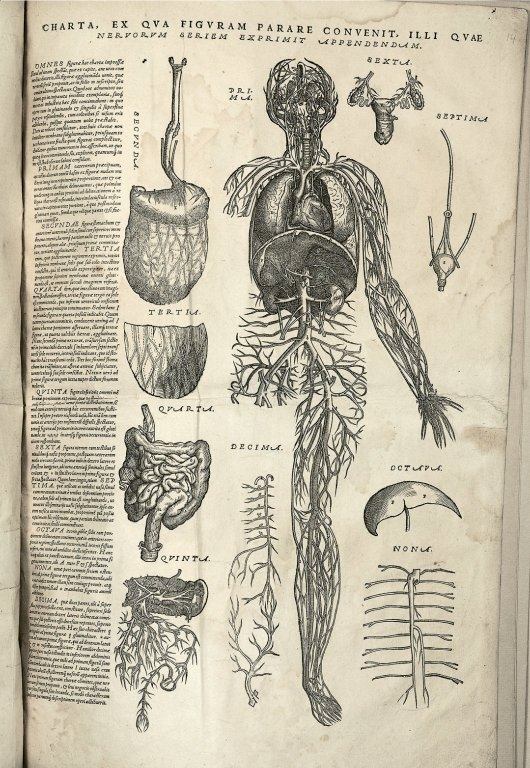
\includegraphics[width=0.25\textwidth]{Anatomia}
    \caption{Ejemplo de anatomía humana.}
    \label{fig:Anatomia}
\end{figure}

Pese a todo, estudiar cuerpos inertes tiene sus limitaciones de modo que durante un tiempo se realizaron vivisecciones para poder comprender mejor como funcionaban todos aquellos órganos, músculos y nervios que ya habían visto con anterioridad. Con el paso del tiempo este sistema fue descartado ya que es una práctica que ponía en peligro la vida del sujeto, haciéndolo pasar por una experiencia terrible en el mejor de los casos.

En la actualidad, gracias al conocimiento acumulado de muchos años y a los avances en otros campos de la ciencia, se han desarrollado dispositivos y técnicas que permiten el estudio en vivo del comportamiento del cuerpo humano de forma no invasiva. Es posible utilizar ecografías para ver el estado del corazón, radiografías para diagnosticar un hueso roto e incluso técnicas más avanzadas como la medicina nuclear que permiten saber que partes del cerebro se activan frente a determinados estímulos sin necesidad de interactuar físicamente con él.

Si bien todas las técnicas anteriores han supuesto auténticos hitos en la medicina moderna y han permitido diagnosticar un gran número de enfermedades así como mejorar la calidad de vida de muchas personas, la mayoría presenta inconvenientes que hacen improbable su uso a nivel personal o docente debido al tamaño de los equipos necesarios para su realización o el coste muy elevado del procedimiento (sin contar con el conocimiento necesario para la realización correcta de la prueba).

Teniendo en mente esta problemática se han desarrollado dispositivos capaces de medir pequeñas las variaciones de voltaje que se producen en el interior de nuestro cuerpo haciendo uso de unos dispositivos denominados electrodos.
\\De esta forma es posible, con un coste muy reducido y un equipamiento relativamente asequible, conseguir inferir que procesos químicos y físicos se están produciendo en el interior de nuestro cuerpo.

Haciendo uso de este sistema y en función del origen de dichas señales dichos registros reciben distintos nombres: electrocardiograma (ECG) para las señales originadas por las contracciones del corazón; electromiograma (EMG) para las generadas en los músculos; electroencefalograma (EEG) para aquellas generadas en el cerebro, etc.

\begin{figure} [H] %this figure will be at the center
    \centering
    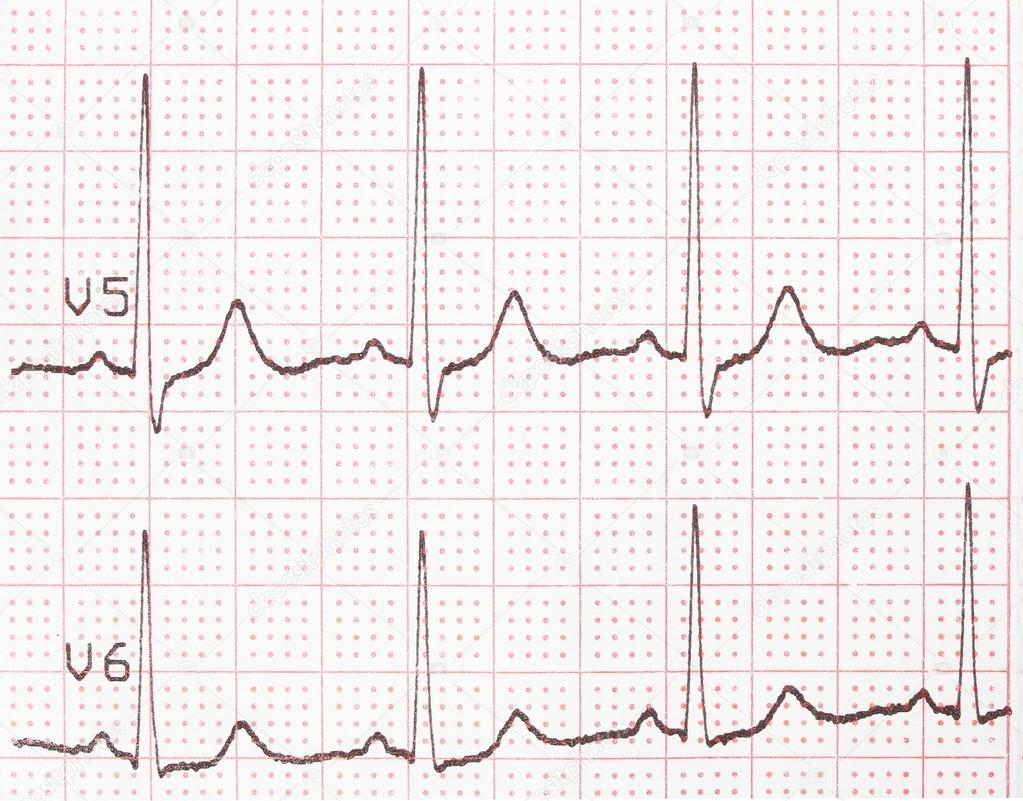
\includegraphics[width=7.5cm]{ECG}
    \caption{Ejemplo de ECG}
    \label{fig:ECG}
\end{figure}

\section{Alcance y estructura del proyecto}
El objetivo de este proyecto es realizar un sistema capaz de captar señales de electroencefalogramas (EEG) manteniendo una buena relación prestaciones/coste. El sistema estará compuesto de dos tarjetas, una de acondicionamiento y de adquisición de datos basada en el circuito integrado ADS1299 y otra de procesamiento y transmisión de dicha información. Esta última es el objetivo del presente proyecto. La plataforma de procesamiento estará basada en un procesador de altas prestaciones, dispondrá de interfaces Wifi, Bluetooth y almacenamiento USB para la transmisión y almacenamiento de los datos respectivamente. 

En la primera fase del proyecto se seleccionará el microcontrolador más adecuado entre los existentes en el mercado analizando características como: capacidad de procesado, interoperación con otros dispositivos, prestaciones...
\\Se compararán los microcontroladores ofrecidos por los distintos fabricantes (ST Microelectronics, Texas instruments, etc) y finalmente, se escogerá aquel que mejor se adecúe a las necesidades del proyecto siendo los principales candidatos los de la familia ARM-M4 STM32F4x por su excelente relación prestaciones-coste.
\\Se valorará también la posibilidad de utilizar diferentes herramientas para la programación del microcontrolador y las alternativas open source en caso de existir.

Una vez hecho el diseño eléctrico de la tarjeta se procederá al diseño de una PCB, la cual se implementará utilizando tecnología SMD en su mayor parte. Para el diseño de la placa se utilizará KiCad por las numerosas ventajas que presenta al ser software libre y la gran cantidad de información que se puede encontrar sobre el funcionamiento del mismo.
Tras depurar la PCB, se implementará un sencillo firmware que permita testear el hardware diseñado y hacer una adquisición básica utilizando la tarjeta SAD utilizando los distintos interfaces implementados.

Adicionalmente se pondrá en marcha un programa para el ordenador basado en LabView donde presentar los datos recibidos.

\section{Base teórica\label{sec:Base_teorica}}

% Documentación interesante para esta sección: 
% http://slideplayer.es/slide/3413933/

Antes de empezar a desarrollar el dispositivo ya mencionado es indispensable realizar una investigación previa del origen de las señales que se quieren adquirir, haciendo especial hincapié en las características de las mismas.

\begin{wrapfigure}[14]{R}{8cm}
    \centering
    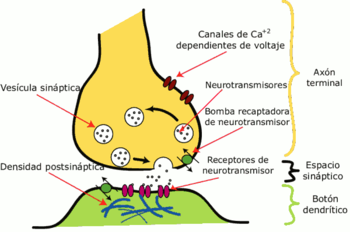
\includegraphics[width=8cm]{Intro_neuronas}
    \caption{Sinapsis neuronal \cite{wikipedia}}
    \label{fig:Intro_neuronas}

\end{wrapfigure}
En el cerebro se realizan \textbf{millones de conexiones} diarias entre las células que la conforman. Dichas células reciben el nombre de \textbf{neuronas}. La comunicación entre ellas se realiza mediante el \textbf{intercambio de neurotransmisores}, proceso que recibe el nombre de sinapsis y que provoca una corriente eléctrica de mayor o menor intensidad que permite la inhibición o activación de las distintas neuronas. 

La suma de todas las corrientes eléctricas conforma lo que se denomina \textbf{actividad bioeléctrica cerebral}. Mediante el uso de sensores es posible medirla y representarla.

Las señales del \acrshort{EEG} dependen del estado de consciencia del usuario y se pueden clasificar en función de su amplitud y frecuencia. Las principales ondas son las siguientes\footnote{Contenido obtenido de \cite{apuntes}}:

\begin{itemize}
\item\textbf{Ondas delta} (hasta 3.5 Hz). Término introducido por W. G. Walter en 1937 para describir a estas ondas de baja frecuencia y alta intensidad (unos centenares de $\mu$V). Tienen lugar en niños de corta edad y en adultos sólo en estado de sueño profundo, inconsciencia o situaciones que aumenten la presión intercraneal como tumores cerebrales.
\end{itemize}
\begin{figure} [H]
    \centering
    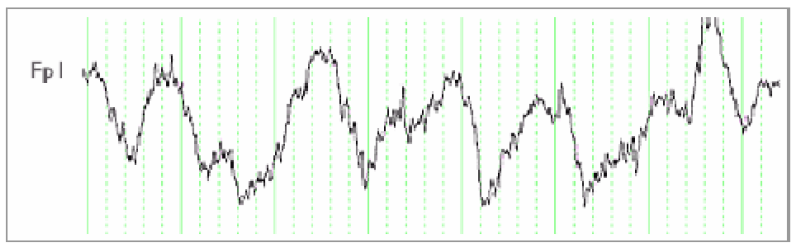
\includegraphics[width=13cm]{ondas_delta}
    \caption{Ondas delta \cite{apuntes}}
    \label{fig:ondas_delta}
\end{figure}

\clearpage

\begin{itemize}
\item\textbf{Ondas theta} (3.5 - 7.5 Hz). Término también Walter aunque mucho más tarde, en 1953. Estas ondas de amplitud inferior a 20 $\mu$ se dan durante el proceso de maduración en toda la corteza cerebral, aunque predomina en la región occipital y temporal y es más rápida en la zona frontal. Dominante en niños entre 5 y 7 años y aún quedan rastros en la juventud. En adultos y adolescentes se asocia a situaciones emocionales y pensamientos de tipo creativo, a estrés o a desordenes psíquicos.
\end{itemize}
\begin{figure} [H]
    \centering
    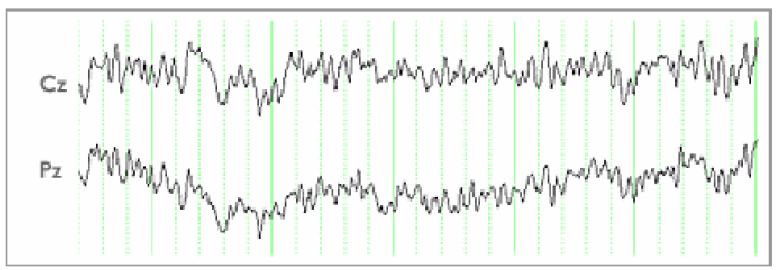
\includegraphics[width=13cm]{ondas_theta}
    \caption{Ondas theta \cite{apuntes}}
    \label{fig:ondas_theta}
\end{figure}

\begin{itemize}
\item\textbf{Ondas alfa} (7.5 - 12.5 Hz). Berger utilizó el término de ritmo alfa para ráfagas de 20-100 $\mu$V de amplitud y gran periodicidad a esas frecuencias predominantes sobre la región occipital pero que aparecen en todo el córtex. Se asocian a estados de relajación, de inactividad y son muy patentes en ausencia de estímulos visuales. Existe mucha variabilidad interpersonal en el ritmo alfa.
\end{itemize}
\begin{figure} [H]
    \centering
    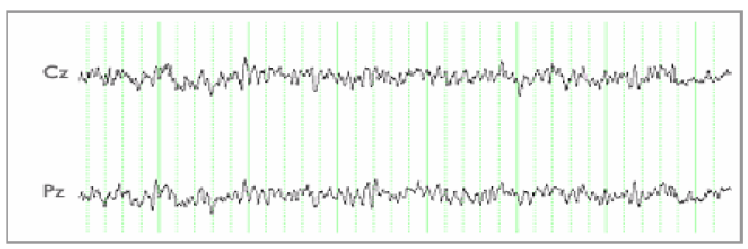
\includegraphics[width=13cm]{ondas_alfa}
    \caption{Ondas alfa \cite{apuntes}}
    \label{fig:ondas_alfa}
\end{figure}

\begin{itemize}
\item\textbf{Ondas beta} (12.5 - 30 Hz). Estas señales de pequeña amplitud, por debajo de 20$\mu$V, son bastante comunes y predominan durante la edad adulta. Suele dividirse en beta baja, beta media y beta alta. El ritmo beta bajo se suele localizar en los lóbulos frontal y occipital y los otros dos están menos localizados. Más irregular que el ritmo alfa, se asocia a actividad psicofísica, estados de agitación, alerta o la actividad mental que se realiza en la resolución de problemas.
\end{itemize}
\begin{figure} [H]
    \centering
    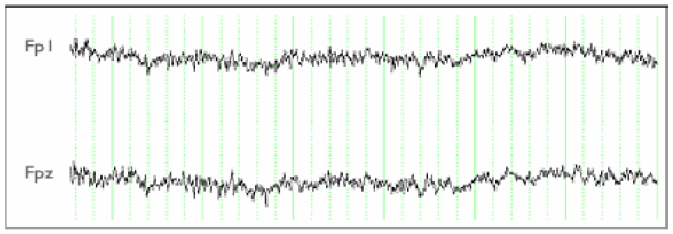
\includegraphics[width=13cm]{ondas_beta}
    \caption{Ondas beta \cite{apuntes}}
    \label{fig:ondas_beta}
\end{figure}

\begin{itemize}
\item\textbf{Ondas gamma} (12.5 - 30 Hz). Esta banda tiene un pico de resonancia, similar a los ritmos alfa, cercano a 40Hz al que se da el nombre de épsilon que se asocia a actividad mental abstracta que interviene en percibir como único por ejemplo el olor, los rasgos de la cara, la personalidad y la voz de una persona. Actualmente hay quien habla de ondas de frecuencias superiores a 50 Hz, son las hipergamma hasta 100 Hz y las lambda hasta 200 Hz, se dice aparecen en los monjes tibetanos en estados de meditación profunda
\end{itemize}

Para la realización de un electroencefalograma existe una disposición estándar en la colocación de los sensores denominada \textbf{sistema 10-20}. Se trata de un sistema internacional que indica la posición en la que se deben colocar los electrodos para una medición del \acrshort{EEG}.  Este sistema separa el cuero cabelludo en torno a un eje Z, colocando los electrodos numerado de manera par a la derecha y los impares a la izquierda (tal y como se puede ver en la figura \ref{fig:colocacion_electrodos)}.

\begin{figure} [H]
    \centering
    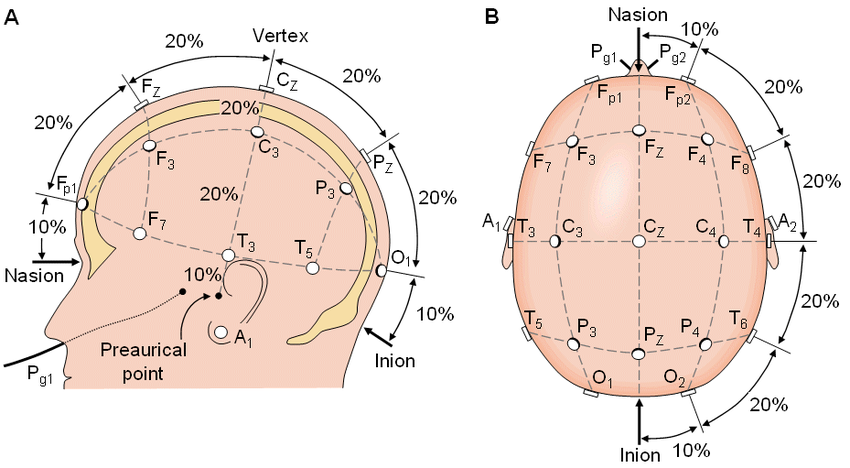
\includegraphics[width=12cm]{colocacion_electrodos}
    \caption{Esquema de colocación de los electrodos}
    \label{fig:colocacion_electrodos}
\end{figure}

\clearpage

\section{Tipos de electrodos\label{sec:Tipos_Electrodos}}

Los electrodos hacen la función de interfaz adaptadora entre los distintos medios por los que se transmiten las señales permitiendo así obtener una señal de mejores características. Este es un funcionamiento similar al de los huesos del oído, pues estos adaptan la señal acústica para que la señal percibida en la coclea tenga unas características determinadas. El funcionamiento de la mayoría de los dispositivos de adquisición de señales en el cuerpo humano depende de estos elementos y hacen uso de dos tipos principales, de trabajo y auxiliar.
\\El electrodo denominado ``de trabajo'' (\textit{working electrode}) es el que adquiere la señal de interés. El otro, denominado auxiliar, es el encargado de crear una referencia. El esquema de la figura \ref{fig:electrodos} muestra un esquema básico de funcionamiento:

\begin{figure} [h]
    \centering
    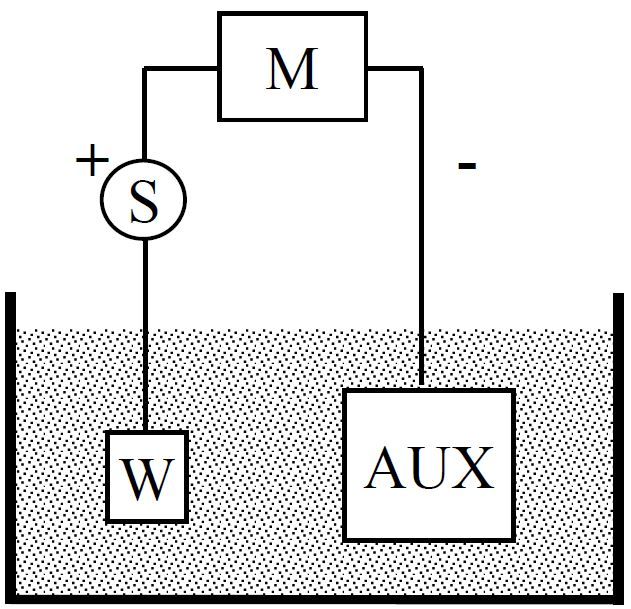
\includegraphics[width=7cm]{electrodos}
    \caption{Electrodos de en un sistema de adquisición \cite{apuntes}}
    \label{fig:electrodos}
\end{figure}

En función del método utilizado por el electrodo para hacer la interfaz con el cuerpo humano estos electrodos se pueden dividir en dos grandes grupos, cada uno con sus ventajas e inconvenientes. 

\subsection{Electrodos húmedos\label{sec:Elec_humedos}}

Los electrodos húmedos se caracterizan por utilizar algún material acuoso para realizar la interfaz entre el dispositivo y el cuerpo humano. Al estar conformados por varios materiales de distinta naturaleza estos electrodos suelen ser de construcción compleja. La figura \ref{fig:electrodo_humedo_2} muestra el esquema de un electrodo húmedo.

\begin{figure} [H]
    \centering
    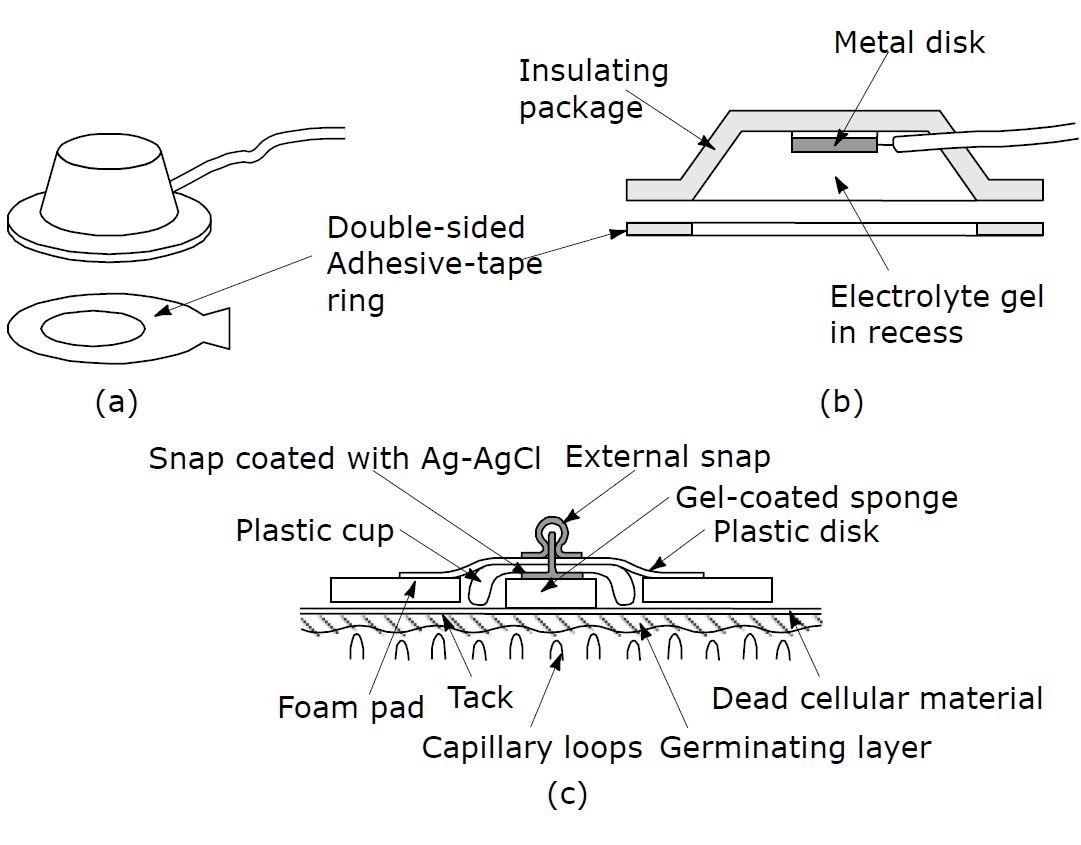
\includegraphics[width=10cm]{electrodo_humedo_2}
    \caption{Esquema de un electrodo húmedo \cite{apuntes}}
    \label{fig:electrodo_humedo_2}
\end{figure}

Estos dispositivos suelen dar muy buen resultado, consiguiendo señales con una buena amplitud y \acrshort{SNR} pero el material utilizado como interfaz suele ser desechable lo que obliga a usar electrodos de usar y tirar o a tener que dedicar mucho tiempo en la preparación y rellenado con gel de la cámara interior del dispositivo. Además, desde el punto de vista de la comodidad del usuario, la utilización de electrodos húmedos puede resultar incómoda al obligarlo a lavar la zona antes y después de su utilización.

La figura \ref{fig:electrodo_humedo_1} muestra un ejemplo de adquisición de \acrshort{EEG} utilizando electrodos húmedos.

\begin{figure} [h]
    \centering
    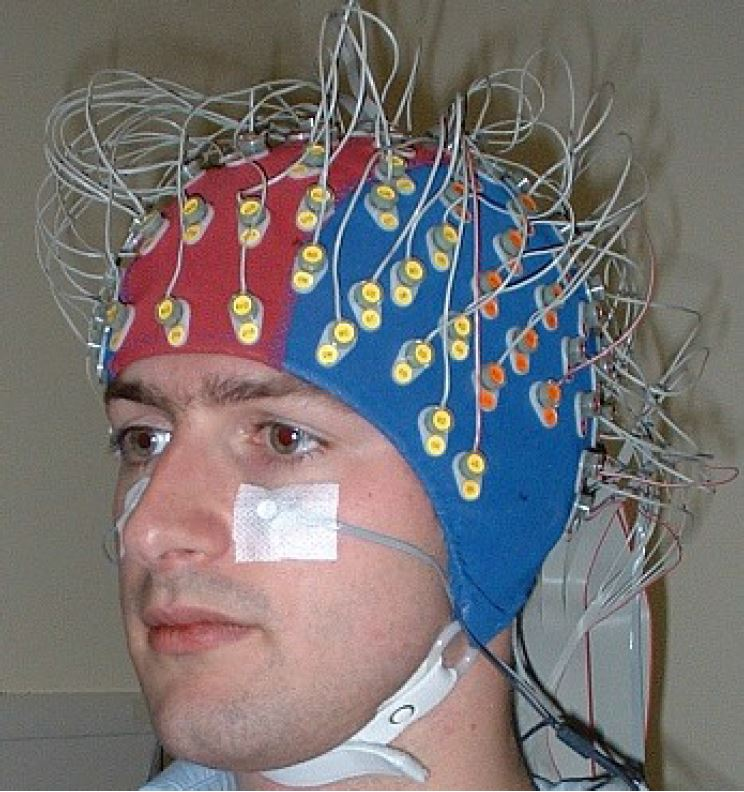
\includegraphics[width=7cm]{electrodo_humedo_1}
    \caption{Medida de un EEG usando electrodos húmedos \cite{apuntes}}
    \label{fig:electrodo_humedo_1}
\end{figure}

\clearpage

\subsection{Electrodos secos\label{sec:Elec_secos}}

Los electrodos secos utilizan materiales sólidos cuya interacción con el cuerpo humano resulta favorable. Al realizar una interfaz con materiales sólidos las señales se transmiten con mayor dificultad, pero este sistema resulta mucho más cómodo para el usuario y los electrodos son de fabricación más sencilla y reutilizables. La figura \ref{fig:electrodo_seco} muestra una representación 3D de un electrodo seco (derecha) y un electrodo seco real junto con sus correspondientes conectores (izquierda).

\begin{figure} [h]
    \centering
    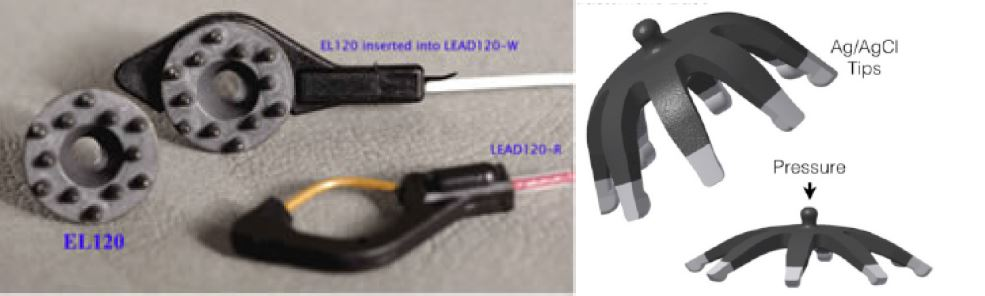
\includegraphics[width=13cm]{electrodo_seco}
    \caption{Electrodo seco real(izquierda) y representación 3D (derecha) \cite{apuntes}}
    \label{fig:electrodo_seco}
\end{figure}

Por comodidad durante la realización de este proyecto se utilizarán principalmente electrodos secos pero la posibilidad de usar electrodos húmedos se mantendrá, pues la utilización de unos u otros afecta al usuario final y a los resultados pero apenas al equipo encargado de su adquisición.

%
% Estado del arte
%
\chapter{Estado del Arte\label{sec:EstadoDelArte}}

Con el paso del tiempo se ha demostrado que una de nuestras mayores virtudes como seres humanos es la habilidad de aprovechar el saber cultivado por otras personas para realizar nuevos descubrimientos con mayor facilidad. En la actualidad con la ayuda de Internet esta ventaja se ha visto potenciada hasta límites insospechados.

Como se ha mencionado con anterioridad en el capítulo \ref{sec:introduccion}, a lo largo de los años se han desarrollado numerosas alternativas a los dispositivos presentes en los hospitales y laboratorios utilizados normalmente para el estudio del cerebro. 
\\Aunque se han invertido muchos recursos en estos dispositivos, el objetivo es permitir ampliar el número de personas capaces de estudiar el cerebro humano, consiguiendo  así aumentar las posibilidades de mejorar nuestro conocimiento sobre el mismo.

De esta forma debería ser más fácil realizar nuevos descubrimientos como, por ejemplo, encontrar nuevas formas de diagnosticar enfermedades o de realizar una comunicación hombre-máquina para aquellas personas que por un motivo u otro no pueden utilizar los medios convencionales.

A lo largo de este capítulo se presentarán algunos de los dispositivos capaces de capturar un EEG haciendo uso de electrodos, algunos a nivel personal, otros enfocados a la docencia y, por supuesto, algunos diseñados por empresas con el fin de realizar un producto final.


Historia procesadores (Gráfica de procesadores)
Antecedentes de la placa (Open BCI)

%
% Diseño
%
\chapter{Diseño\label{sec:diseño}}

Este proyecto consiste en una ampliación y cambio de enfoque de otro proyecto llevado a cabo de manera simultánea por una alumna de la Universidad Politécnica de Madrid llamada Nerea Urrestarazu que a su vez se basa en el Kit de demostración de rendimiento del ADS1299 proporcionado por Texas Instrument.

\begin{figure} [h]
    \centering
    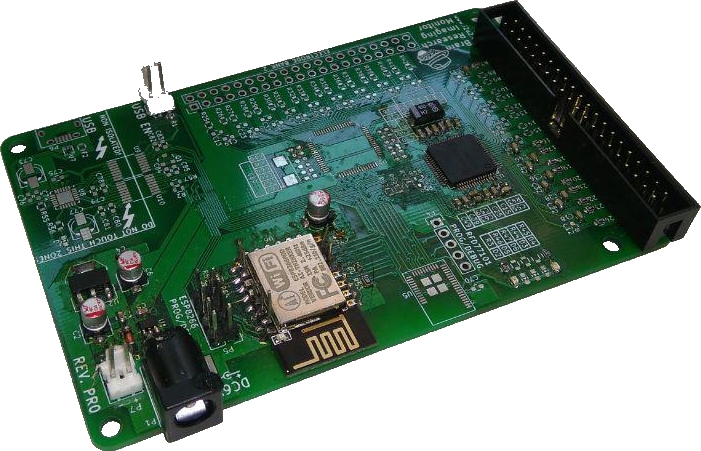
\includegraphics[width=7cm]{Placa_Nerea}
    \caption{Placa final del proyecto base}
    \label{fig:Placa_base}
\end{figure}

\section{Diseño base\label{sec:Diseno_base_N}}

El proyecto original trata sobre el diseño y desarrollo de una placa de adquisición de EEG haciendo uso de los integrados ADS1299 junto con un sistema de transmisión hacia el ordenador tanto inalámbricamente como a través de USB. La figura \ref{fig:Diseno_base} muestra las partes que componen dicho diseño.

\begin{figure} [h]
    \centering
    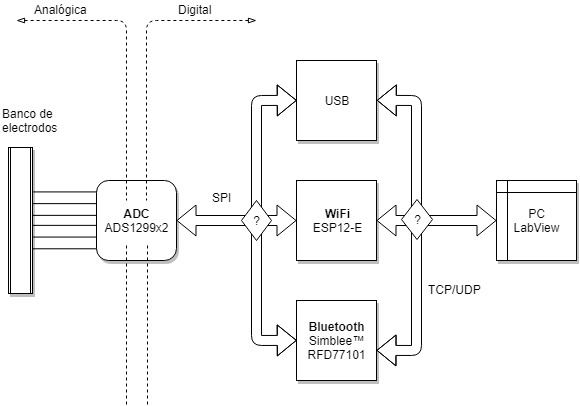
\includegraphics[width=12cm]{Esquema_diseno_base}
    \caption{Esquema del proyecto base}
    \label{fig:Diseno_base}
\end{figure}

\subsection{Adquisición de datos\label{sec:Adquisicion_N}}

La parte encargada de la adquisición está compuesta por un par de bancos de electrodos dispuestos en los laterales de la placa seguidos de un filtro paso-bajo con frecuencia de corte de 6.79kHz encargado de eliminar las componentes de frecuencias muy altas, no deseadas en el estudio de un \acrshort{EEG}. A continuación se encuentran conectados a sus respectivos bancos los \acrshort{ADC} ADS1299. 
\\Estos convertidores son capaces de adquirir información de forma independiente o en modo ``Daisy Chain'' y transmitirla a través de \acrshort{SPI} hacia otros dispositivos cuya misión será gestionarla.

\begin{figure} [h]
    \centering
    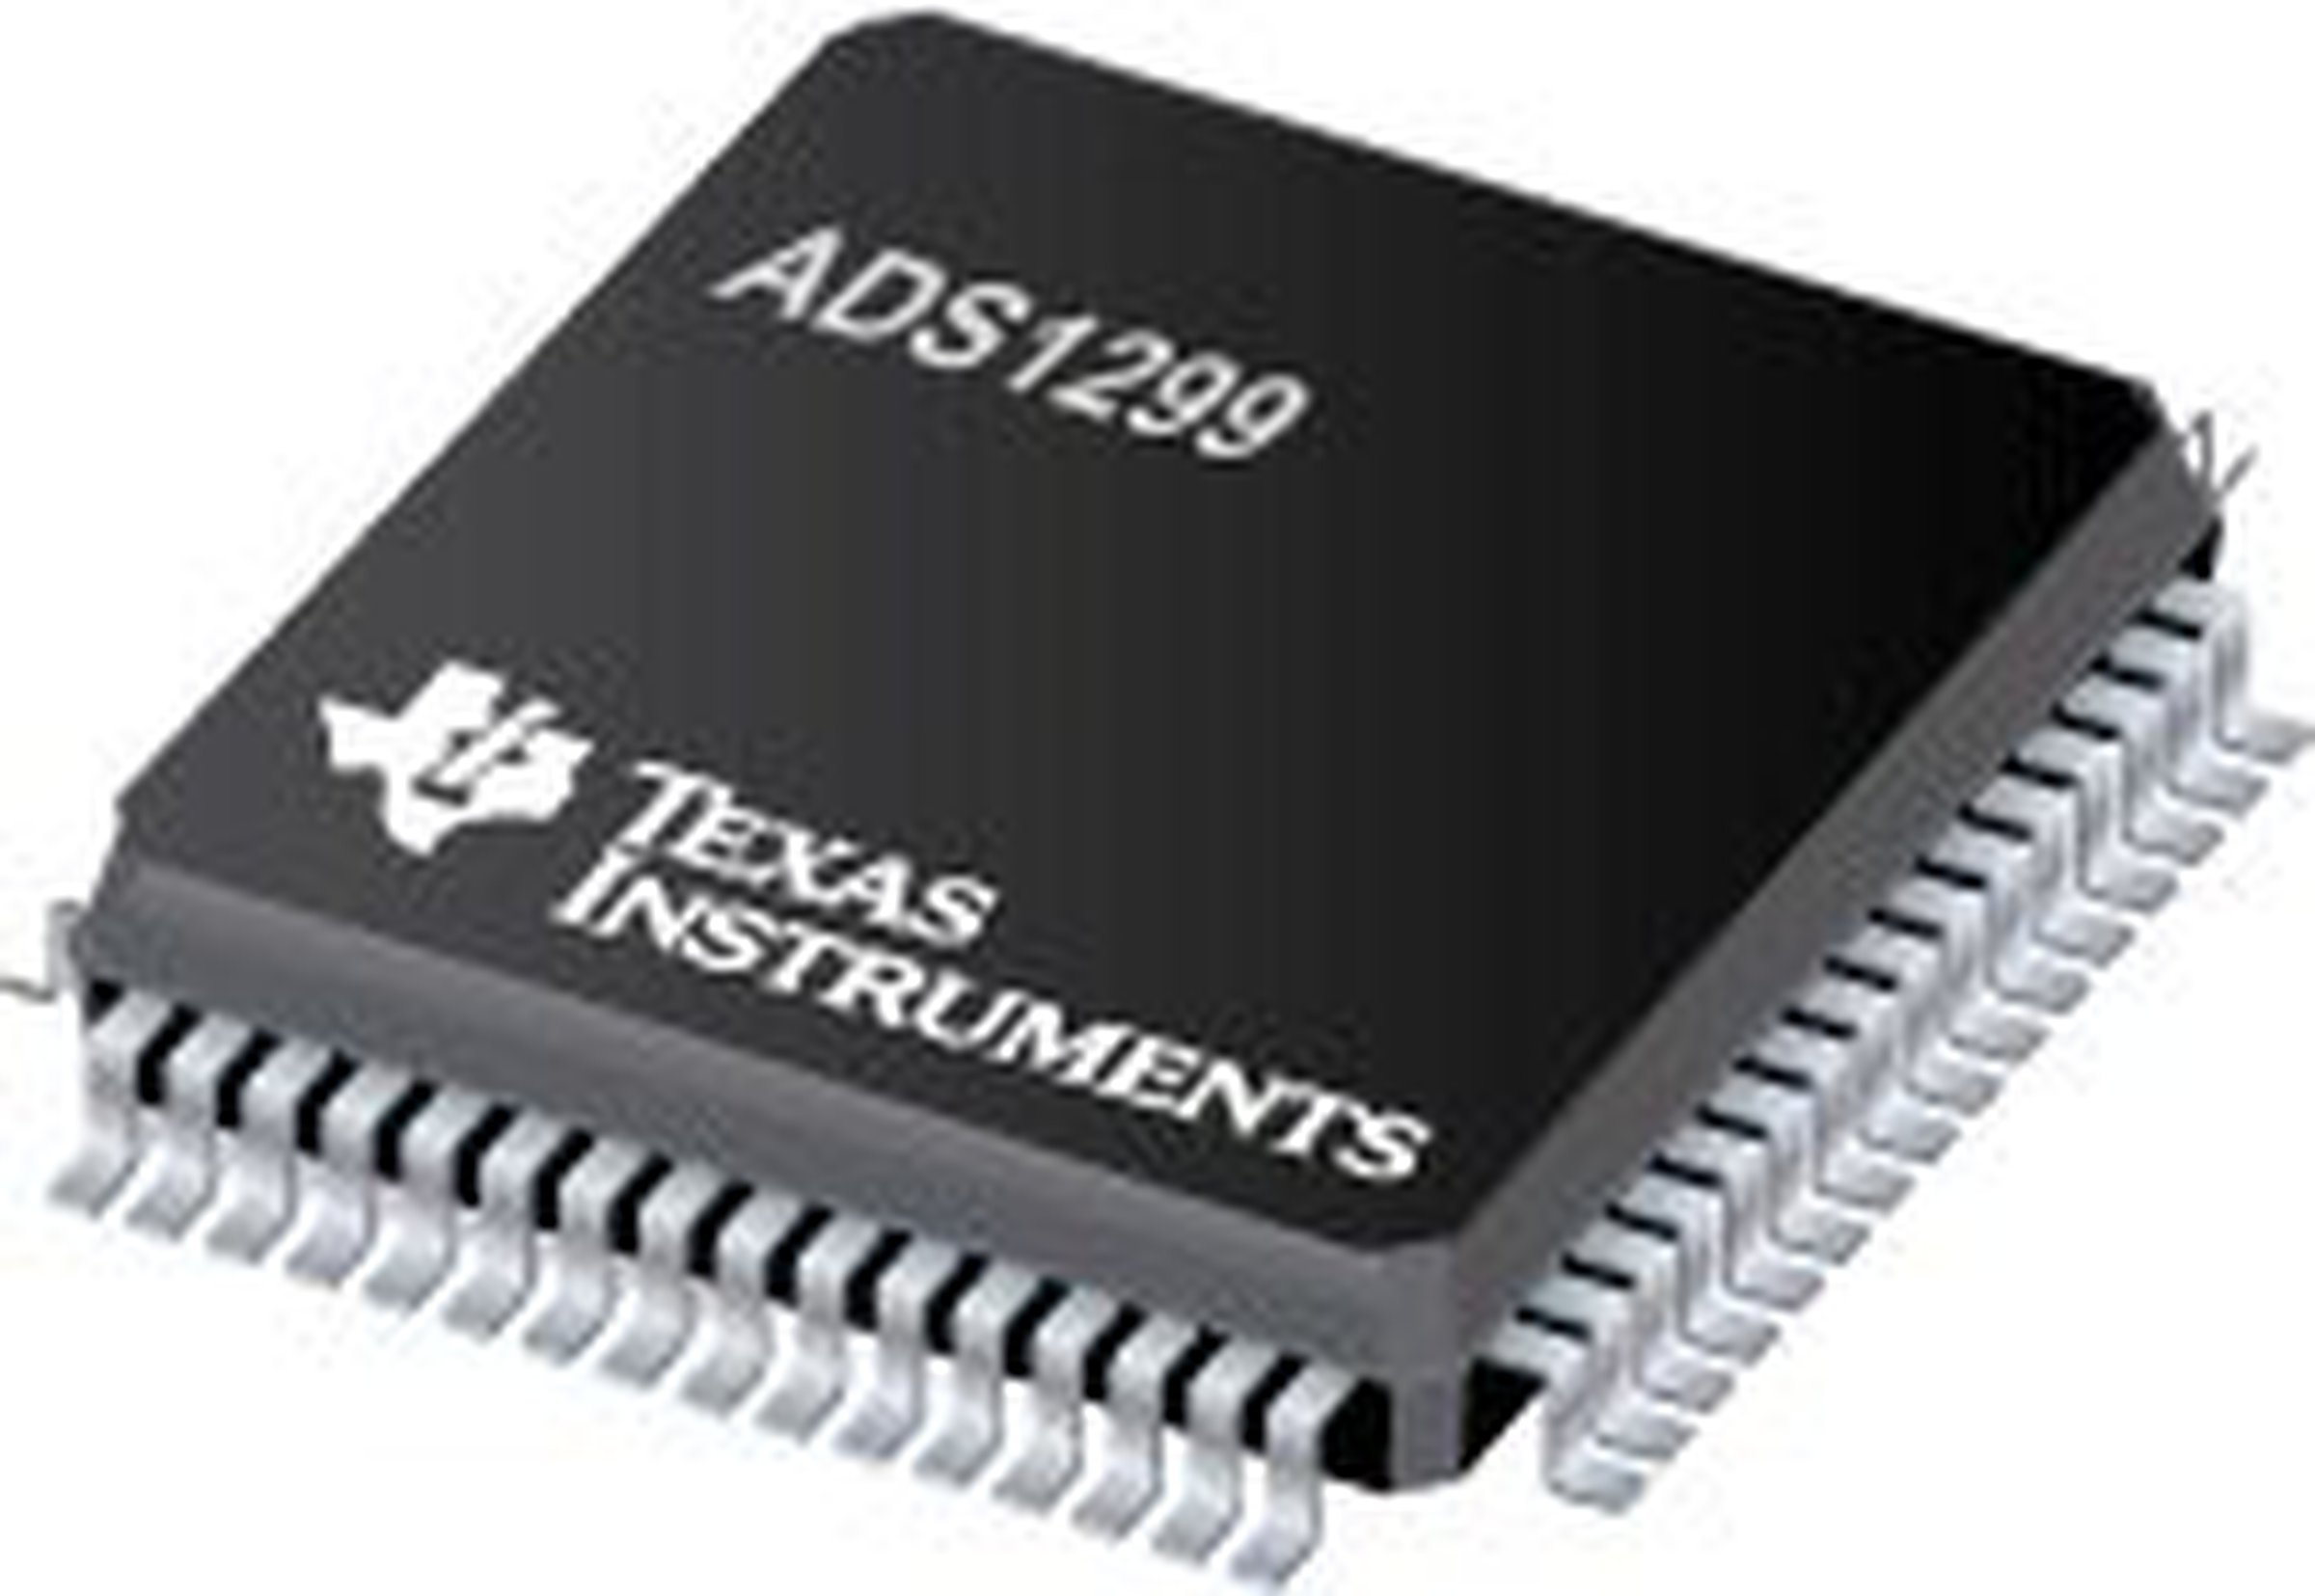
\includegraphics[width=6cm]{ADS1299}
    \caption{Convertidor Analógico-Digital ADS1299}
    \label{fig:ADS1299}
\end{figure}

El \acrshort{SPI} presente en el convertidor permite leer todos los registros del ADS y escribir la gran mayoría. Aunque normalmente se leen los relacionados con los datos convertidos, también es posible saber el estado de los \acrshort{GPIO} o el identificador único del dispositivo leyendo su registro asociado.

La configuración del ADS se realiza mediante la escritura de ciertos registros, cada uno asociado a un parámetro específico. La tabla \ref{tab:Conf_Reg_ADS} muestra los registros disponibles, tanto de lectura como de configuración, una descripción básica y la dirección de memoria asociada a los mismos.

\begin{table} [h]
    \centering
    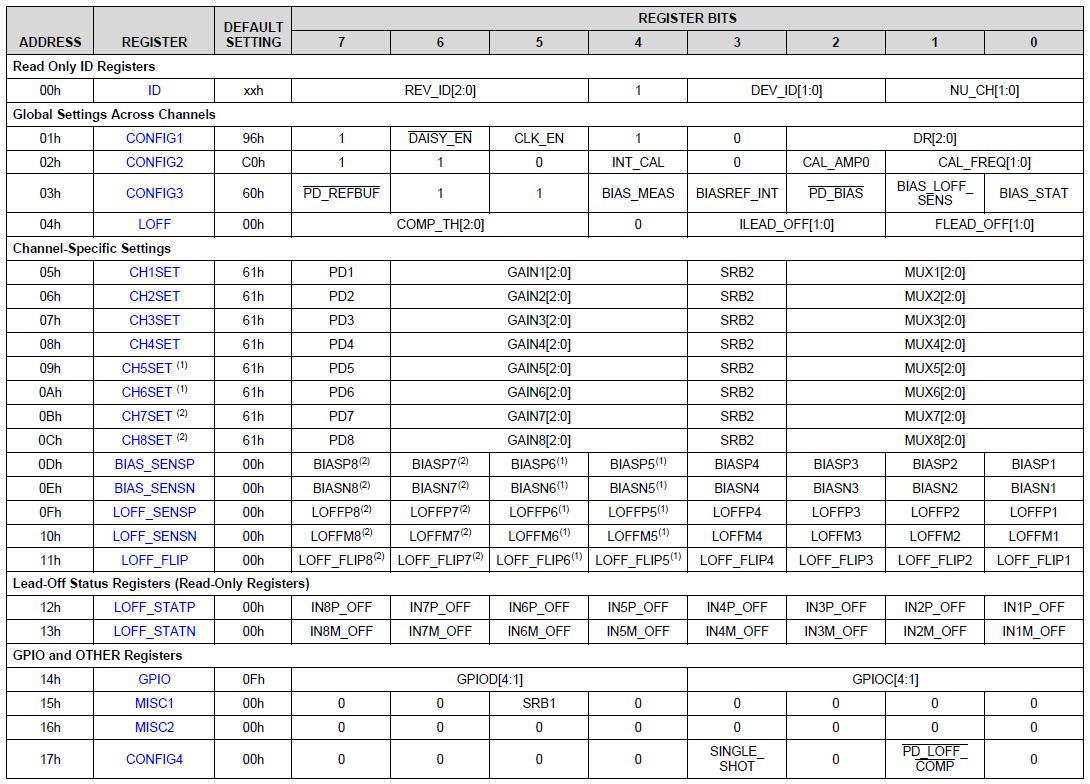
\includegraphics[width=\textwidth]{Tabla_registros_ADS}
    \caption{Tabla de registros de la familia ADS}
    \label{tab:Conf_Reg_ADS}
\end{table}

Una descripción más detallada de cada uno de los bits de cada registro se puede encontrar en el \textit{datasheet} del componente\cite{Datasheet_ADS}.

Como se puede ver en la tabla \ref{tab:Conf_Reg_ADS}, los convertidores cuentan con una gran cantidad de opciones de configuración. Para el desarrollo de este proyecto se ha implementado un sistema de configuración que permite la lectura y escritura de todos los registros.

\subsection{Transmisión de datos\label{sec:Transmisión_N}}

Tras completar el proceso de adquisición de datos resulta necesario transmitir dicha información hacia un dispositivo capaz de procesarla. Para ello la placa original contaba con dos alternativas. La primera consiste en, mediante \acrshort{USB} y acopladores aislantes, transmitir la información a un ordenador. 
\\La segunda hace uso de dos tecnologías inalámbricas distintas que funcionan de forma excluyente y son seleccionables con un \textit{jumper}: WiFi o Bluetooth.

\subsubsection{WiFi\label{sec:WiFi_N}}

Para la transmisión de datos a través de WiFi se seleccionó el módulo ESP12-E, basado en el \acrshort{SoC} ESP2866, también conocido nodemcu.
\\Este cuenta con un microcontrolador (\acrshort{MCU}) embebido de 32 bits (Tensilica L106) con una memoria \acrshort{RAM} de 36kB y una velocidad de reloj de la \acrshort{CPU} de hasta 80MHz, proporcionando suficiente potencia para las tareas básicas.

Así mismo se incluye montado en el mismo paquete una memoria flash de 4MB en la que almacenar el código de los programas que se ejecutarán y una antena embebida, dotando al módulo de conectividad en la banda de 2.4GHz.

\begin{figure} [h]
    \centering
    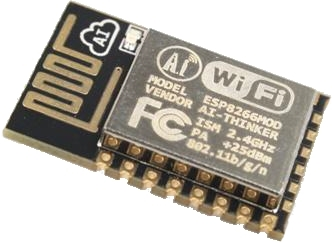
\includegraphics[width=6cm]{ESP8266}
    \caption{ESP8266}
    \label{fig:ESP8266}
\end{figure}

A efectos de diseño es muy importante saber cuales serán las entradas/salidas del dispositivo así como los pines dedicados para su programación. La figura \ref{fig:ESP8266_pinout} muestra un resumen de todas las funciones de cada uno de los pines. Como se puede observar, el \acrshort{SPI} hace uso de los pines 5, 6, 7 y 16. Por otro lado el \acrshort{UART}, necesario para la programación del micro hace uso de los pines 16 y 17. Dichos pines deberán reservarse posteriormente en la fase de diseño de la \acrshort{PCB}.

El dispositivo tiene tres modos de arranque dependiendo del sitio desde el que cargue el código y la selección de uno u otro modo viene determinada por los pines MTDO, GPIO0 y GPIO2. \\La tabla \ref{tab:ESP_Boot_Modes} resume los distintos modos de arranque así como el estado en el que debe estar cada uno de los pines para entrar en ese modo.
\begin{table} [h]
 	\centering
	\begin{tabular}{|c|c|c|c|c|}
		\hline 
		MTDO & GPIO0 & GPIO2 & Modo & Descripción \\ 
		\hline 
		L & L & H & UART & Descarga el código desde UART \\ 
		\hline 
		L & H & H & Flash & Carga desde memoria Flash a través de SPI \\ 
		\hline 
		H & x & x & SDIO & Carga desde una tarjeta SD \\ 
		\hline 
	\end{tabular} 
	\caption{Modos de arranque del ESP12-E\cite{ESP_Boot_mode}}
    \label{tab:ESP_Boot_Modes}
\end{table}	

\clearpage

\begin{figure} [h]
    \centering
    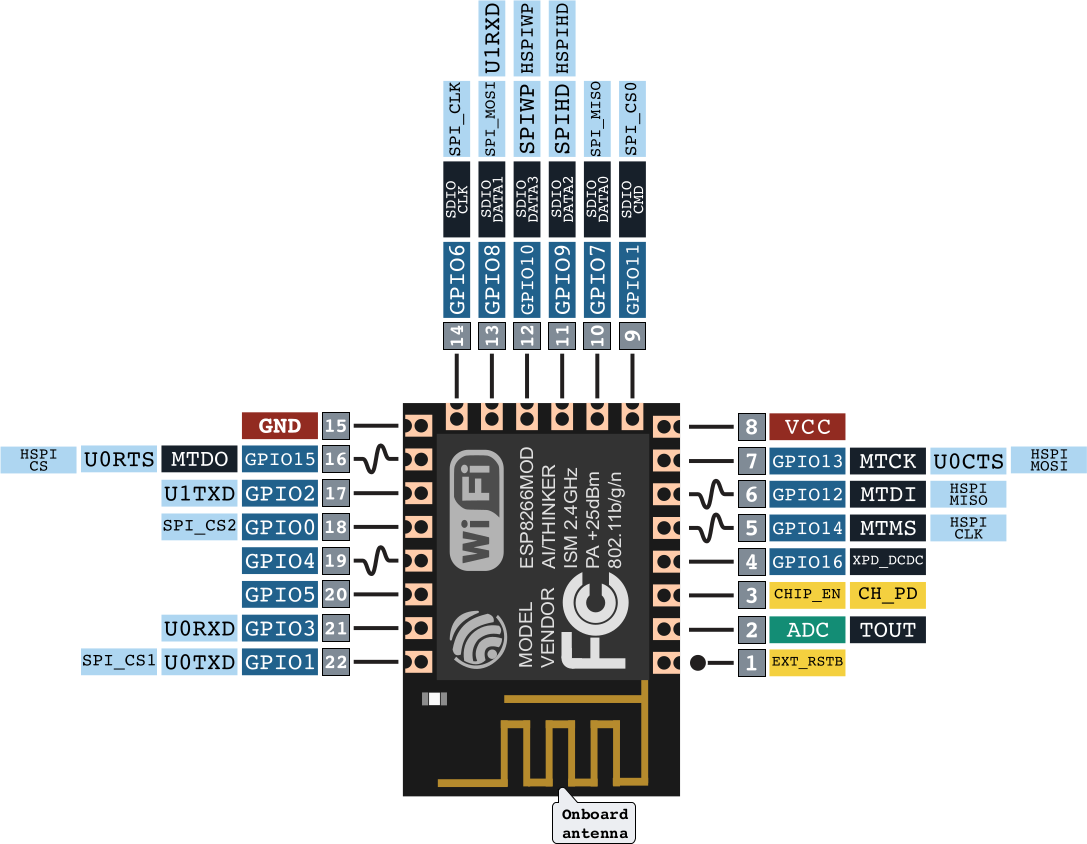
\includegraphics[width=\textwidth]{esp8266-esp12e-pinout}
    \caption{Resumen de todas las Entradas/Salidas del ESP12-E\cite{ESP_Pinout}}
    \label{fig:ESP8266_pinout}
\end{figure}

\subsubsection{Bluetooth\label{sec:Bluetooth_N}}

Para la transmisión de datos a través de Bluetooth se seleccionó el módulo Simblee™ RFD77101 ya que al igual que el módulo WiFi, cuenta con interfaces de comunicación a través de \acrshort{SPI} para conectarse con el \acrshort{ADC} (pines 21, 22, 31 y 32) y de \acrshort{UART} para su programación posterior programación (pines 23 y 24).

\begin{figure} [H]
    \centering
    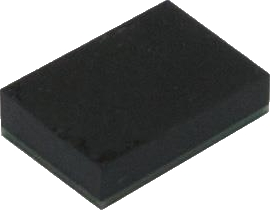
\includegraphics[width=5cm]{BT}
    \caption{Simblee™ RFD77101}
    \label{fig:BT}
\end{figure}

El módulo presenta un ARM Cortex-M0 como \acrshort{CPU} con 128KB de memoria Flash, 24KB de \acrshort{RAM} y una frecuencia de reloj de 16MHz. 

Todos los dispositivos de transmisión inalámbrica anteriormente mencionados permiten su programación utilizando el \acrshort{IDE} de Arduino lo cual facilita sensiblemente el proceso de desarrollo y prototipado teniendo la ventaja adicional de que es Software Libre.


\subsubsection{USB\label{sec:USB_N}}


Como este proyecto tiene como objetivo independizar el sistema lo máximo posible del ordenador se ha optado por desestimar el sistema de transmisión por \acrshort{USB} conservando solamente la interfaz inalámbrica. 

\section{Diseño final\label{sec:Diseño_final}}
          
Llegados a este punto se han analizado las características más importantes de cada uno de los elementos presentes en el sistema original, siendo los más importantes las distintas interfaces de comunicación y los pines de programación.
\\Con esta información ya es posible independizar cada uno de esos elementos y crear un nuevo diseño que cumpla con las especificaciones de este nuevo proyecto.

\begin{figure} [h]
    \centering
    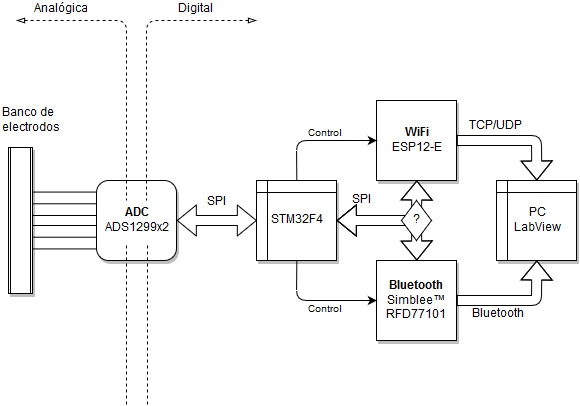
\includegraphics[width=12cm]{Esquema_proyecto_Javier}
    \caption{Esquema del proyecto final}
    \label{fig:Esquema_proyecto_Javier}
\end{figure}

El nuevo sistema estará compuesto por tres partes:
\begin{itemize}
\item En primer lugar etapa de adquisición compuesta de un banco de electrodos con sus correspondientes filtros analógicos y dos \acrshort{ADC}. 
\item Posteriormente un microcontrolador se encargará de realizar el procesado de la señal y la gestión de los distintos elementos.
\item Por último la transmisión de datos se realizará de forma inalámbrica a un ordenador u otro dispositivo mediante Bluetooth o WiFi.
\end{itemize}

Como se puede observar en la figura \ref{fig:Esquema_proyecto_Javier}, el ordenador sigue estando presente en el sistema pero en esta ocasión su función se limita a mostrar la información siendo fácilmente sustituible en un futuro por un dispositivo menos potente y barato. Al utilizar un microcontrolador en la propia placa de adquisición se consigue aumentar la independencia del sistema y se dota de unas características muy interesantes, tanto de procesado de señal como de almacenaje de la misma o gestión del consumo.

\subsection{Selección del microcontrolador\label{sec:Sel_micro}}

El microcontrolador es el núcleo del sistema. Para poder interactuar con todos los elementos anteriormente descritos deberá contar con las siguientes características:
\begin{itemize}
\item Bajo precio.
\item Bajo consumo.
\item Capacidad procesado de señal.
\item Para poder utilizar el máximo de la velocidad de adquisición de los ADS (16k\acrshort{SPS}) y evitar cuellos de botella, deberá contar con un Bus SPI de al menos 5.85Mb/s dedicados para la transmisión y la misma cantidad para recepción o dos buses.
\[Tasa\ de\ transferencia = 16k\ Muestras/s * 8\ canales * 24bits * 2\ ADS = 5.85Mb/s\]

\end{itemize}

Hay una gran cantidad de microcontroladores en el mercado que podrían utilizarse para este proyecto pero, de entre todos los disponibles, aquellos con arquitectura \textbf{ARM} son los que mejor se adaptan a las especificaciones. Concretamente los más adecuados son aquellos englobados en la familia \textbf{Cortex M4} ya que están especialmente diseñados con \acrshort{DSP} integrado para conseguir un rendimiento máximo minimizando el consumo.

\begin{figure}[h]
  \begin{subfigure}[b]{0.49\textwidth}
   	\centering
    
\includegraphics [height=2.5cm]{Texas_Instument}
    \caption{Logo de Texas Instument}
    \label{fig:Logo_TI}
  \end{subfigure}
  \hfill
  \begin{subfigure}[b]{0.49\textwidth}
  	\centering
    
\includegraphics[height=2.5cm]{STMicroelectronics}
    \caption{Logo de STMicroelectronics}
    \label{fig:Logo_STM}
  \end{subfigure}
  \caption{Principales fabricantes contemplados}
\end{figure}

\clearpage

La tabla \ref{tab:Comparativa_MCU} muestra varios dispositivos de esa familia vendidos por Texas Instrument o STMicroelectronics y un resumen de sus características principales.
\begin{table} [h]
	\centering
	\begin{tabular}{|c|c|c|c|c|}
\hline 
 &\multicolumn{2}{c|}{Texas Instruments}& \multicolumn{2}{c|}{STMicroelectronics} \\ 
\hline 
 & TM4C123GH6PM & TM4C1294NCPDT & STM32F405& STM32F469  \\ 
\hline 
\acrshort{FCPU} [MHz] & 80 & 120 & 168 & 180 \\ 
\hline 
Flash [kB] & 256 & 1024 & 1024 & 2048 \\ 
\hline 
\acrshort{RAM} [kB] & 32 & 256 & 192 & 384 \\ 
\hline 
\acrshort{SPI} & x4 & x4 & x2 + 1 & x6 \\ 
\hline 
Precio [€] & 8,72 & 12,74 & 9,24 & 13,48 \\ 
\hline 
	\end{tabular} 
	\caption{Comparativa entre distintos MCUs}
	\label{tab:Comparativa_MCU}
\end{table}

Todos los dispositivos anteriormente contemplados tienen \acrshort{DSP} integrados así como una Unidad de Punto Flotante (\acrshort{FPU}) que permite realizar operaciones matemáticas avanzadas de forma óptima.

Entre los dispositivos anteriores, los pertenecientes a la familia STM presentan mejor relación coste/prestaciones, pero el verdadero factor diferenciador son las herramientas dispuestas para la comunidad por parte del fabricante.
\\En la página web se pueden encontrar distintas herramientas y PDFs que facilitan sensiblemente el proceso de desarrollo para esta plataforma. 

Finalmente se seleccionó el \acrshort{MCU} STM32F405 en el formato \acrshort{LQFP64} ya que sus características se ajustan perfectamente a las especificaciones, manteniendo unas muy buenas prestaciones y un precio bastante bajo. Todo esto con el valor añadido de que ya se contaba con la placa de desarrollo STM32F4 Discovery lo cual permitió comenzar con el aprendizaje y estudio del entorno sin la necesidad de esperar al diseño, impresión y soldado de la placa final.

\begin{figure} [h]
    \centering
    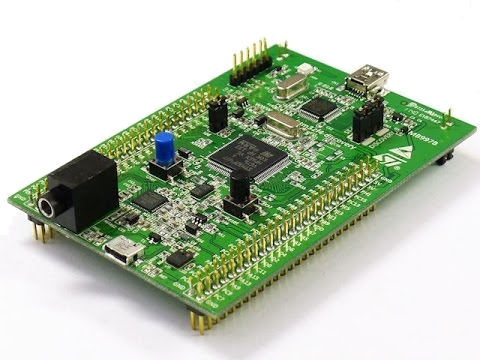
\includegraphics[width=5cm]{STM32F4_Discovery}
    \caption{Placa de desarrollo STM32F4 Discovery}
    \label{fig:STM32F4_Discovery}
\end{figure}

El \acrshort{MCU} cuenta con 3 buses SPI independientes que pueden funcionar en modo \textit{\gls{Full Duplex}}. El SPI$_1$  es capaz de funcionar hasta 42Mb/s mientras que los SPI$_2$ y SPI$_3$ pueden comunicar información hasta 21Mb/s. Los pines dedicados a dichos buses se pueden consultar en el \textit{Datasheet} del componente\cite{Datasheet_STM}.
\\Otra característica interesante de este \acrshort{MCU} es la presencia de forma nativa de un gestor de \acrshort{USB} \acrlong{OTG} (\acrshort{OTG}) permitiendo así conectar un dispositivo \acrshort{USB} para almacenar información a largo plazo.

\clearpage

\subsection{Alimentación\label{sec:Alimentación}}

Tras seleccionar todos los elementos se va a proceder a escoger una alimentación que permita a todos los dispositivos funcionar en condiciones óptimas.
\\La tabla \ref{tab:Alimentacion} muestra un resumen de todos los elementos presentes en el sistema junto con los rangos de voltaje recomendados por los fabricantes para su alimentación.

\begin{table} [h]
	\centering
	\begin{tabular}{|c|c|c|}
	\hline 
	Dispositivo & V$_{min}$ [V] & V$_{max}$ [V] \\ 
	\hline 
	Simblee BT & 1.8 & 3.6 \\ 
	\hline 
	ESP12-E & 3.0 & 3.6 \\ 
	\hline 
	STM & 1.8 & 3.6 \\ 
	\hline 
	ADS (Digital) & 1.8 & 3.6 \\ 
	\hline 
	ADS (Analógica) & 4.75 & 5.25 \\ 
	\hline 
	USB & 5 & 5 \\ 
	\hline 
	\end{tabular} 
	\caption{Rangos de alimentación de todos los elementos}
	\label{tab:Alimentacion}
\end{table}

De la tabla \ref{tab:Alimentacion} se deduce que para que todos los dispositivos funcionen correctamente será necesario dotar a la placa de 5 voltios con los que se podrá alimentar la parte analógica del ADS así como el USB mientras que la parte digital se puede alimentar en el rango de 3V a 3.6V. 

Por motivos de compatibilidad con el diseño anterior y tras comprobar que se cumple con los requisitos impuestos por los nuevos elementos del sistema se ha optado por mantener el mismo esquema de alimentación que en el proyecto base.

El sistema de alimentación se compone de dos partes principales, cada una encargada de proporcionar el voltaje deseado manteniendo el ruido generado por el mismo al mínimo.

\subsubsection{Alimentación 3.3V\label{sec:Alimentacion_3.3V}}
Para conseguir un voltaje de 3.3V estable se ha utilizado el regulador AZ1117C-3.3 ya que es capaz de conseguir una precisión para el voltaje de salida del $\pm$1\% así como un ruido de salida de 0.003\% V$_{out}$ entre 10Hz y 10kHz.
En la figura \ref{fig:Alim_3.3} se muestra el esquema eléctrico utilizado, que es una variación del circuito recomendado por el fabricante en su \textit{datasheet}\cite{Datasheet_3.3}.

\begin{figure} [h]
    \centering
    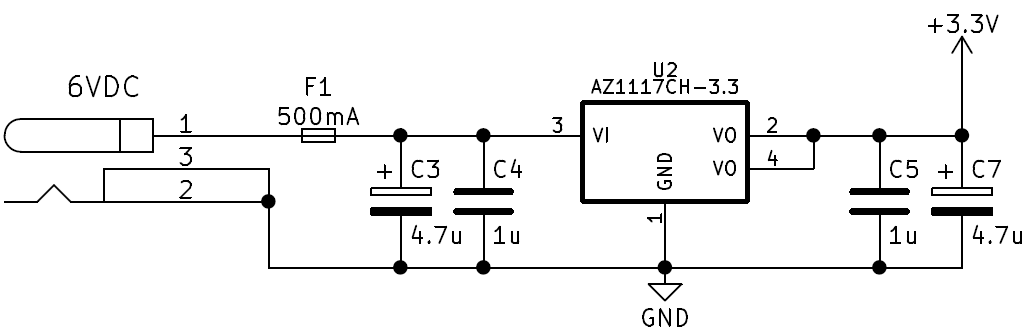
\includegraphics[width=10cm]{Alim_3_3}
    \caption{Esquema de alimentación a 3.3V}
    \label{fig:Alim_3.3}
\end{figure}

\subsubsection{Alimentación 5V\label{sec:Alimentacion_5V}}

Los 5V serán utilizados por el dispositivo de almacenamiento USB para su alimentación y por el ADS para generar los distintos voltajes de referencia que necesita para operar correctamente. Al afectar de forma directa a las mediciones realizadas por el ADS la eliminación de variaciones en este voltaje es crucial, pues estas supondrán un ruido añadido a la señal final.

El regulador encargado de proporcionar 5V es el MCP1711. Este integrado está caracterizado por tener un rizado de salida menor al 1\% del voltaje de salida así como de poseer una corriente en reposo muy baja. Este último parámetro facilitará el diseño de un sistema portátil alimentado por baterías aumentando la duración de la misma. La figura \ref{fig:Alim_5} muestra el esquema eléctrico utilizado.

\begin{figure} [h]
    \centering
    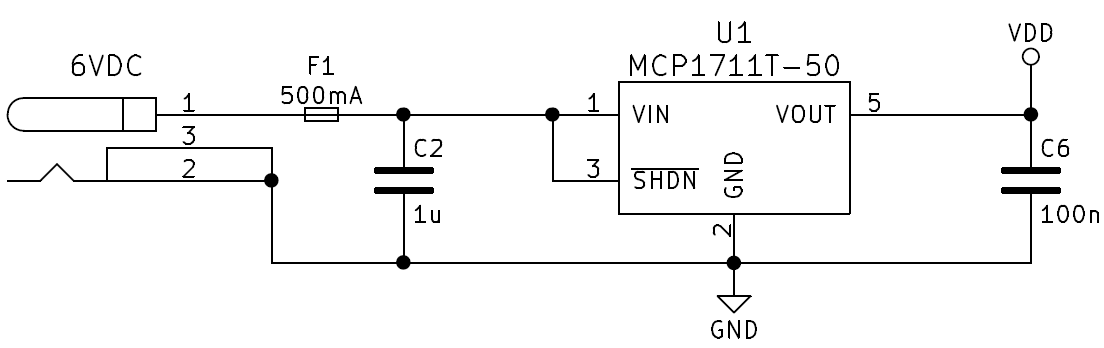
\includegraphics[width=10cm]{Alim_5}
    \caption{Esquema de alimentación a 5V}
    \label{fig:Alim_5}
\end{figure}

Para funcionar correctamente ambos integrados necesitan que el voltaje de entrada sea superior al voltaje de salida en un factor que en la documentación técnica recibe el nombre de ``\gls{Tensión de Dropout}''(V$_{DROP}$).
\\De acuerdo al Datasheet de ambos reguladores, V$_{DROP}$ es para 3.3V y 5V, 1.3V y 0.43V respectivamente. Con esa información se deduce que el integrado que limita el diseño es el regulador de 5V así como que con una entrada de al menos 5.43V ambos reguladores deberían funcionar correctamente.

Finalmente se ha optado por una fuente de alimentación de 6V ya que esto permitirá hacer uso de pilas o baterías para alimentar el sistema, dotándolo de independencia de la red eléctrica y eliminando el riesgo de electrocución.

\clearpage

\section{Circuito electrónico y esquemáticos\label{sec:Esquemáticos}}

El último paso de la fase de desarrollo será generar un esquemático capaz de englobar todos los elementos anteriormente presentados, interconectarlos y dar como resultado un sistema funcional.

En este punto es importante valorar dos alternativas de diseño, cada una con sus ventajas e inconvenientes: Implementación de todo el circuito de cero o crear una placa que se conecte a la ya existente.

Si bien es cierto que para un diseño final crear una placa que englobe todos los componentes sería lo ideal, pues presentaría un formato más compacto y mejor presentación, hacerlo también supone crear una placa más grande y desaprovechar aquellas ya construidas en proyectos anteriores.

Teniendo en cuenta que se cuenta con varias placas ya montadas y que el sistema está en fase de prototipo, se va a optar por la segunda opción, creando una segunda placa independiente en la que se incluirán todos los elementos correspondientes a la gestión de las señales digitales del sistema, dejando las señales analógicas en la otra placa. De esta forma la fase de diseño de la \acrshort{PCB} y de montaje se simplifica considerablemente y se abaratan costes al reutilizarse componentes.

Para la conexión con la otra placa se aprovechará el espacio dejado por el módulo ESP12-E, pues al hacer uso de \acrshort{SPI} es posible obtener todas las señales necesarias para interactuar con el ADS.

El sistema embebido en esta placa incluirá los elementos que se pueden ver en la figura \ref{fig:Esquematico_global}

\begin{figure} [h]
    \centering
    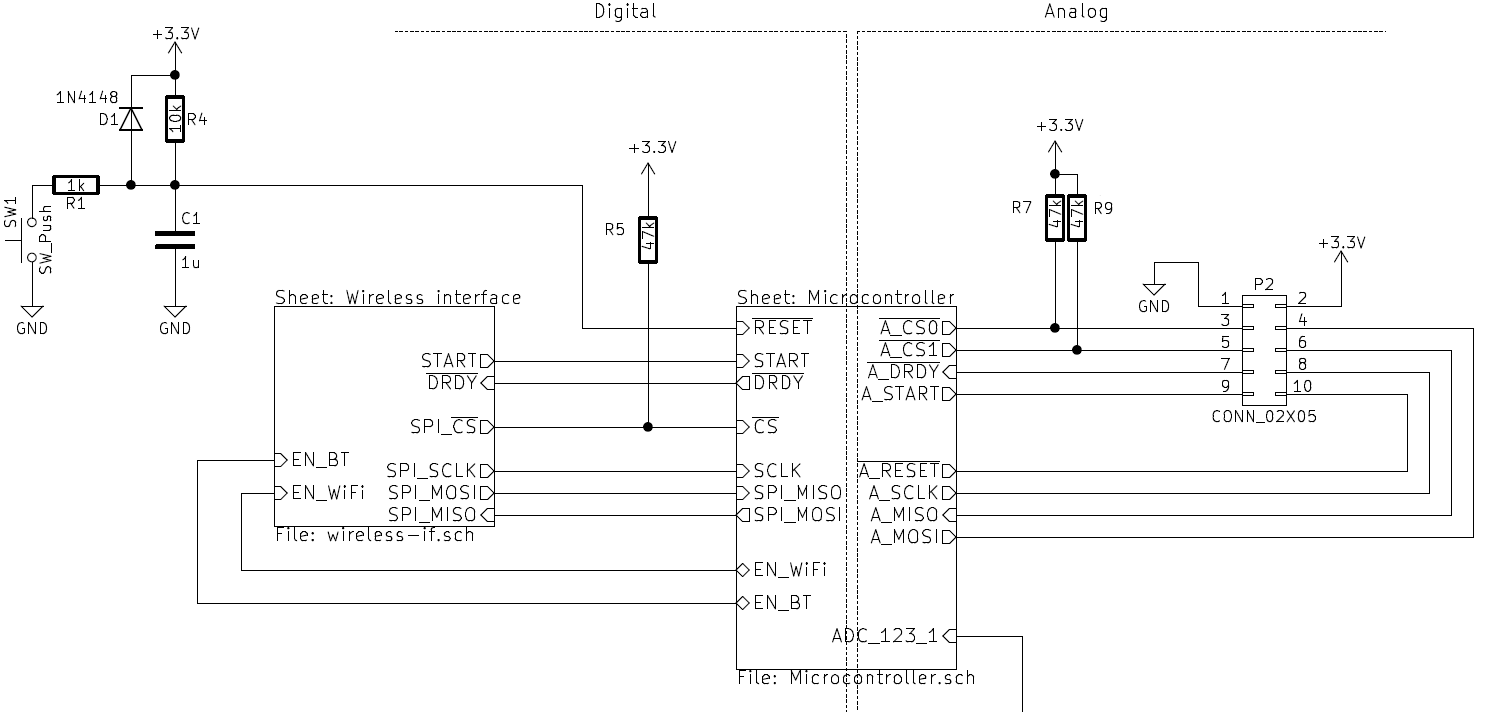
\includegraphics[width=14cm]{Esquematico_global}
    \caption{Esquema general del sistema}
    \label{fig:Esquematico_global}
\end{figure}

Se ha incluido en la placa un botón de reinicio con su correspondiente circuito electrónico así como una realimentación desde la alimentación hasta uno de los pines \acrshort{ADC} el microcontrolador para poder monitorizar el estado de la batería.

\subsection{Circuito de alimentación\label{sec:Esquemáticos_alim}}

Aunando los dos circuitos presentados en la sección \ref{sec:Alimentación} el resultado final es el obtenido en la figura \ref{fig:Alim_final}.

\begin{figure} [h]
    \centering
    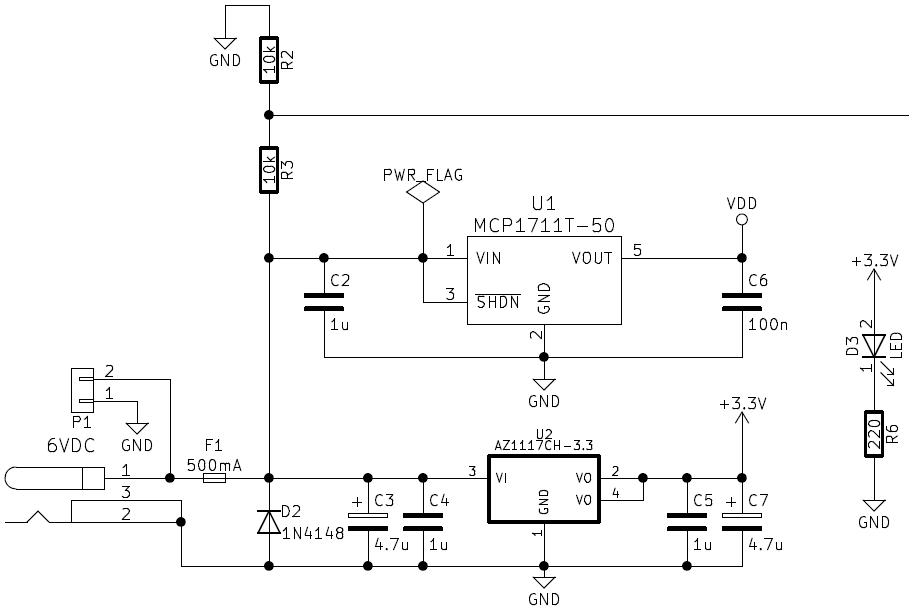
\includegraphics[width=14cm]{Alim_final}
    \caption{Esquemático final del circuito de alimentación}
    \label{fig:Alim_final}
\end{figure}

El fusible (F1) garantiza que la máxima corriente que consumirá el dispositivo es de 500mA, evitando así que el sistema o el paciente sufran daños en caso de un cortocircuito. Adicionalmente se ha incluido un diodo \acrshort{LED} cuya función es indicar el estado de la placa. Si la placa ha encendido correctamente o si se encuentra en funcionamiento el \acrshort{LED} se encenderá.

El diodo (D2) junto con el condensador (C3) evitarán que los transitorios afecten al voltaje de entrada asegurando así que la alimentación que recibirán ambos integrados será lo más estable posible.

Con el objetivo de monitorizar el estado de la batería se ha utilizado el \acrshort{ADC} incorporado en el propio microcontrolador. Como la señal de entrada se encuentra fuera del rango soportado en las especificaciones del STM se ha optado por incorporar las resistencias R2 y R3 formando un divisor de tensión utilizando así la señal resultante para realizar las medidas.

\clearpage

\subsection{Microcontrolador\label{sec:Esquemáticos_micro}}

El microcontrolador es el núcleo del sistema. Este hace de centro de control de todas las señales digitales que se transmiten así como de gestor de dispositivos, decidiendo que dispositivos se encuentran activos en cada momento. 
Para gestionar que dispositivos se encuentran habilitados se ha sustituido el \textit{jumper} de la placa original por \acrshort{GPIO} del microcontrolador. De esta forma se consigue mayor flexibilidad, automatización y se optimiza el consumo. 

Adicionalmente se ha integrado un \acrshort{LED} conectado al pin PA9 que dotará a la placa de indicadores visuales del estado en el que se encuentra.

La figura \ref{fig:Esquematico_micro} muestra una representación del integrado así como todos los elementos con los que está conectado.

\begin{figure} [h]
    \centering
    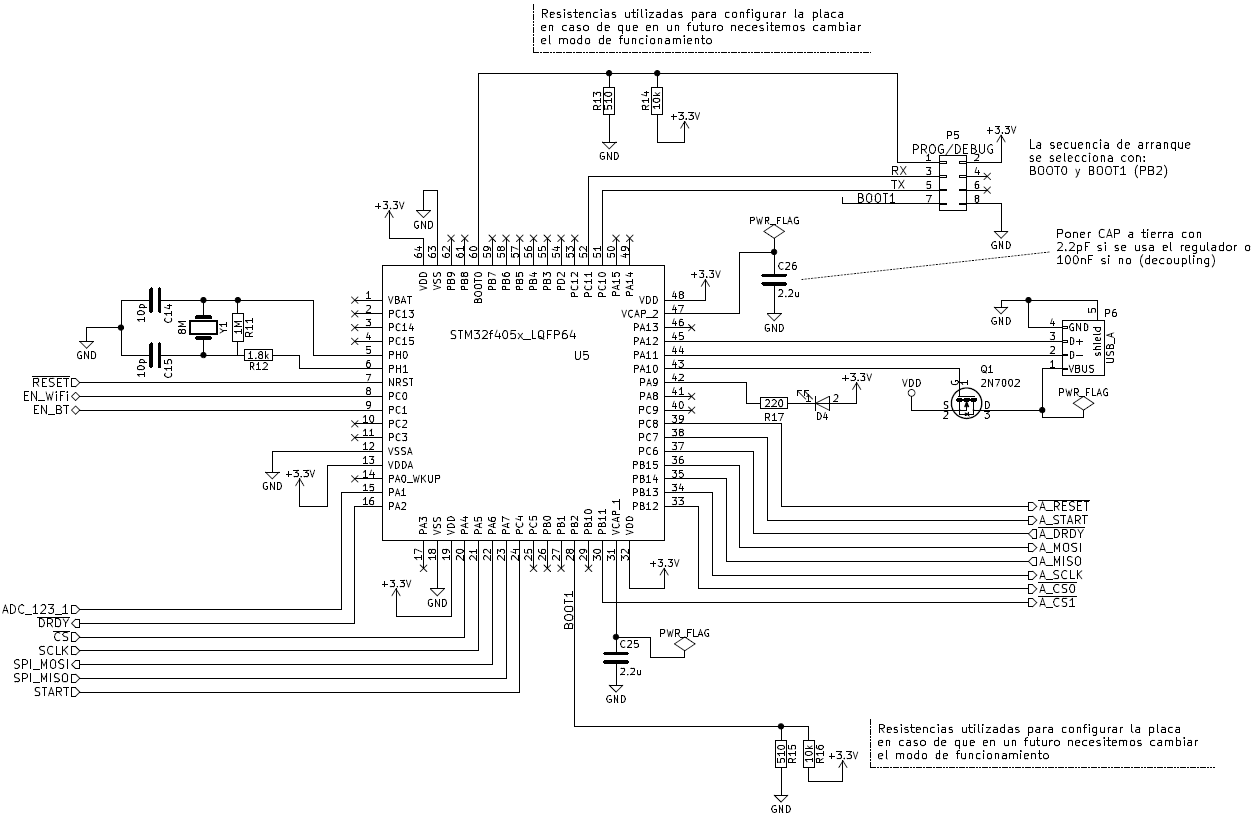
\includegraphics[width=\textwidth]{Esquematico_micro}
    \caption{Esquemático del microcontrolador}
    \label{fig:Esquematico_micro}
\end{figure}

El modo de arranque del dispositivo viene determinado por el estado de los pines Boot0 y Boot1. Haciendo uso de las resistencias R13, R14, R15 y R16 se consigue forzar que en condiciones normales de operación el STM arranque desde la memoria Flash integrada. 
\\Con el objetivo de reprogramar el microcontrolador se ha añadido el conector P5. Dicho conector permite alternar entre los distintos modos de arranque del STM así como interactuar con el por UART. Esta última característica será la que permitirá subir el código a ejecutar pero también brinda funciones de \textit{debug}.

\clearpage

El sistema aprovecha dos de los 3 buses \acrshort{SPI}. El bus SPI1, capaz de transmitir a 41Mb/s se ha reservado para la comunicación ESP12-E $\Longleftrightarrow$ STM32F4 mientras que el utilizado para comunicarse con los ADS es el SPI2 con una velocidad de hasta 21Mb/s.

El \acrshort{MCU} puede trabajar con un oscilador interno sin problemas pero la presencia de un oscilador externo basado en un cristal de cuarzo proporciona ciertas ventajas como son mayor precisión en el reloj y la posibilidad de usar \acrshort{PLL} para aumentar la frecuencia de trabajo del procesador.
\\El circuito asociado al cristal se puede observar en la parte superior izquierda de la figura \ref{fig:Esquematico_micro} pero se incluye a continuación para facilitar la lectura de este documento:

\begin{figure} [h]
    \centering
    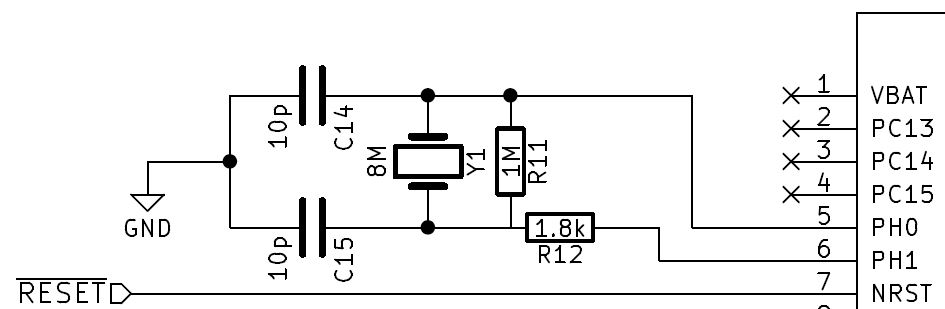
\includegraphics[width=10cm]{Detalle_cristal}
    \caption{Detalle del circuito asociado al oscilador externo}
    \label{fig:Detalle_cristal}
\end{figure}


Para realizar un diseño funcional del circuito del oscilador se ha utilizado el \textit{datasheet} del dispositivo junto con una guía de buenas prácticas\cite{Guia_Oscilador}, ambos proporcionados por el fabricante. La configuración utilizada a nivel de software para la gestión de dicho reloj se explicará en mayor profundidad en el capítulo \ref{sec:Implementacion}.

Se han añadido todos los condensadores recomendados por el fabricante. Algunos deben tener una capacidad determinada en función del modo de funcionamiento del microcontrolador (C25 y C26), otros, denominados condensadores de desacoplo, tienen como objetivo eliminar el ruido de altas frecuencias de la zona de alimentación. El condensador C11 es denominado Bulk y tiene como objetivo garantizar una alimentación lo más estable posible.

\begin{figure} [h]
    \centering
    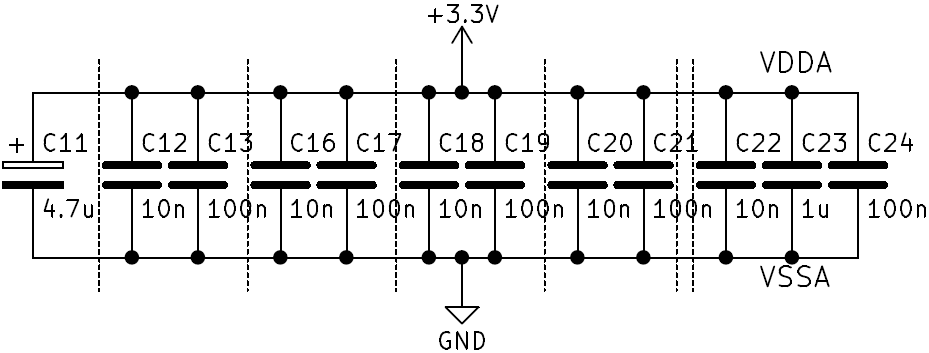
\includegraphics[width=10cm]{Condensadores_micro}
    \caption{Condensadores Bulk (C11) y de desacoplo}
    \label{fig:Condensadores_micro}
\end{figure}

 Por simplicidad y legibilidad se han agrupado todos en una zona del esquemático pero a la hora de diseñar la PCB será necesario tener presente que para que el dispositivo funcione correctamente estos últimos deben localizarse lo más cerca posible de los pines de alimentación.

Finalmente, como el \acrshort{MCU} tiene la capacidad de interactuar directamente con dispositivos \acrshort{USB}, con el objetivo de implementar en un futuro características que aprovechen dicha capacidad se ha añadido un conector \acrshort{USB} cuyo bus de alimentación se encuentra controlado por el propio \acrshort{MCU}. De esta forma es posible habilitar y deshabilitar el dispositivo USB y reducir el consumo.



%
% Implementación
%
\chapter{Implementación de la PCB\label{sec:Implementacion_PCB}}

TODO: Implementación

Hardware
	PCB (Añadir BOM)
	
	Primeras pruebas y programación
	

	
	

\chapter{Implementación del software\label{sec:Implementacion_soft}}

Una vez finalizado el soporte físico del sistema, será necesario implementar a nivel de software todas las funciones deseadas.

El sistema está compuesto por tres microcontroladores, cada uno de ellos con sus propias características y métodos de programación. Debido a esto, a lo largo de este capítulo se explicará con detenimiento el software utilizado individualmente para ellos así como los distintos entornos de desarrollo (\acrshort{IDE}) necesarios.

Los distintos elementos se presentarán siguiendo el mismo orden que la información que se desea adquirir. Este es:
ADS $\Rightarrow$ Microcontrolador $\Rightarrow$ Interfaz inalámbrica $\Rightarrow$ PC.

\section{Microcontrolador STM32F4\label{sec:Software_micro}}

Debido a la complejidad de los microcontroladores de la familia STM32, los desarrolladores han dedicado su tiempo y esfuerzo en crear herramientas que faciliten su programación. Estas herramientas llamadas \acrshort{IDE} contienen una recopilación de funciones, utilidades y ejemplos que simplifican sensiblemente el proceso de diseño e implementación del software que ejecutará el microcontrolador.

Es tan grande la comunidad de desarrolladores que hay detrás del STM que numerosas empresas han visto como una oportunidad de negocio la creación de un \acrshort{IDE} propietario.

\clearpage

\begin{figure} [h]
    \centering
    
\includegraphics[width=13cm]{STM32_IDEs}
    \caption{IDEs alternativos disponibles \cite{STM32_IDEs}}
    \label{fig:STM32_IDEs}
\end{figure}

La figura \ref{fig:STM32_IDEs} muestra algunos entornos de desarrollo recomendados por el fabricante en su propia página web. Como se puede apreciar, en la imagen se hace distinción entre las opciones comerciales (azul) y las gratuitas (verde).

Uno de los objetivos de este proyecto era utilizar Software Libre en la medida de lo posible. Por ese motivo se probaron algunas de las alternativas presentes en la imagen anterior dando preferencia a aquellas basadas en Oracle como ``System Workbench for STM32'' (AC6). A continuación se presentan algunas de las utilizadas al comienzo del proyecto junto con sus características y el motivo de su descarte:
\begin{itemize}
   \item \textbf{CooCox}\\
   Presenta muchos ejemplos prácticos pero su interfaz es muy lenta. Necesita demasiado tiempo para iniciar.
   \item \textbf{Arduino}\\
   Fase muy temprana de desarrollo.
   \item \textbf{System Workbench for STM32}
   \\Buena comunidad pero incompatible con las herramientas de STM.
\end{itemize}

\begin{figure} [h]
    \centering
    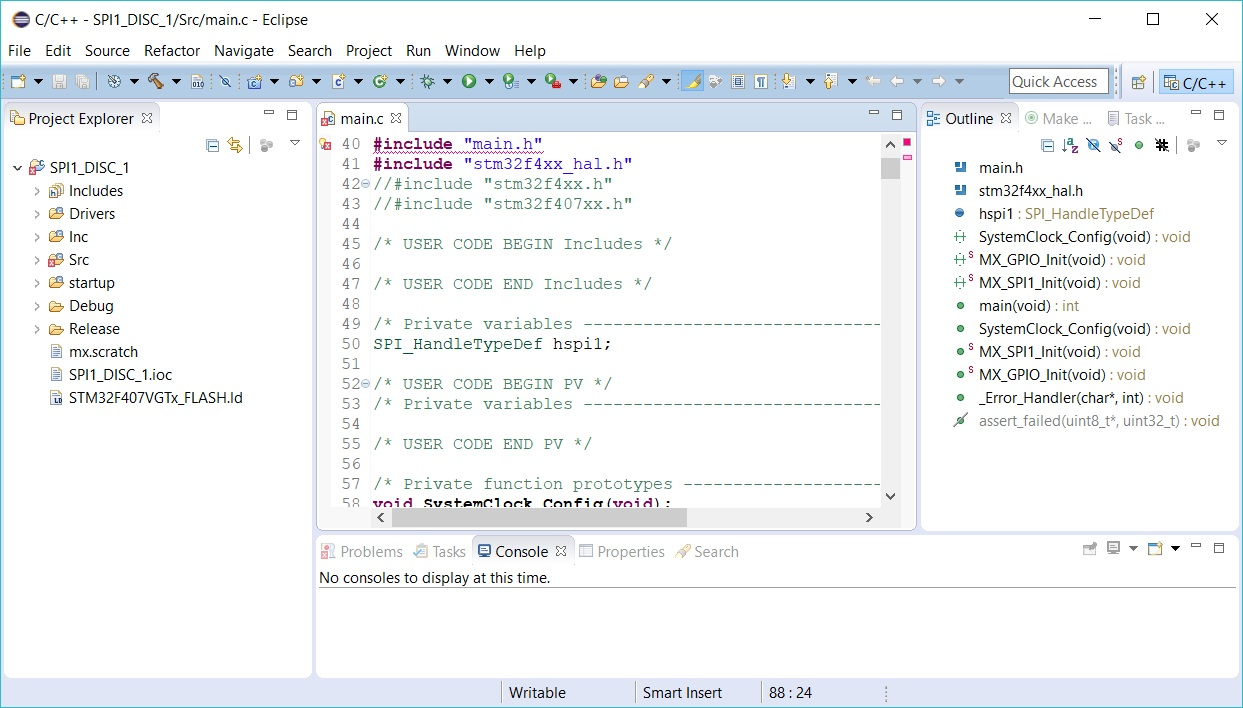
\includegraphics[width=12cm]{Alternative_IDE}
    \caption{Ejemplo de IDE alternativo}
    \label{fig:Alternative_IDE}
\end{figure}

Finalmente se optó por armKeil, pues tiene una gran cantidad de ejemplos y librerías descargables desde la propia interfaz, contiene un gran número de funciones adicionales y la compatibilidad con las herramientas de STM es muy buena. Aunque en la figura \ref{fig:STM32_IDEs} aparece entre las alternativas gratuitas se debe destacar que cuenta con dos versiones, una gratuita que permite realizar proyectos básicos y otra comercial destinada a aplicaciones de mayor envergadura. La limitación de la versión gratuita consiste en forzar un tamaño máximo de programa de 32KB. Si el código a compilar supera dicha longitud directamente no compilará.

\subsection{Configuración inicial\label{sec:Configuracion_micro}}

Aunque Keil permite comenzar un proyecto utilizando como base algunos de los ejemplos que contiene, la configuración de las características del microcontrolador (reloj, interfaces, etc.) puede resultar una tarea muy compleja y tediosa, incluso para aquellos desarrolladores más experimentados. Con el objetivo de facilitar esta tarea, el fabricante ha creado un software con interfaz amigable que permite configurar de forma gráfica el procesador llamado STM32CubeMX que hace uso de un conjunto de elementos y \textit{drivers} llamado \acrshort{HAL} que se explicará con más detalle al comienzo del apartado \ref{sec:Software_micro_HAL}.

\begin{figure} [h]
    \centering
    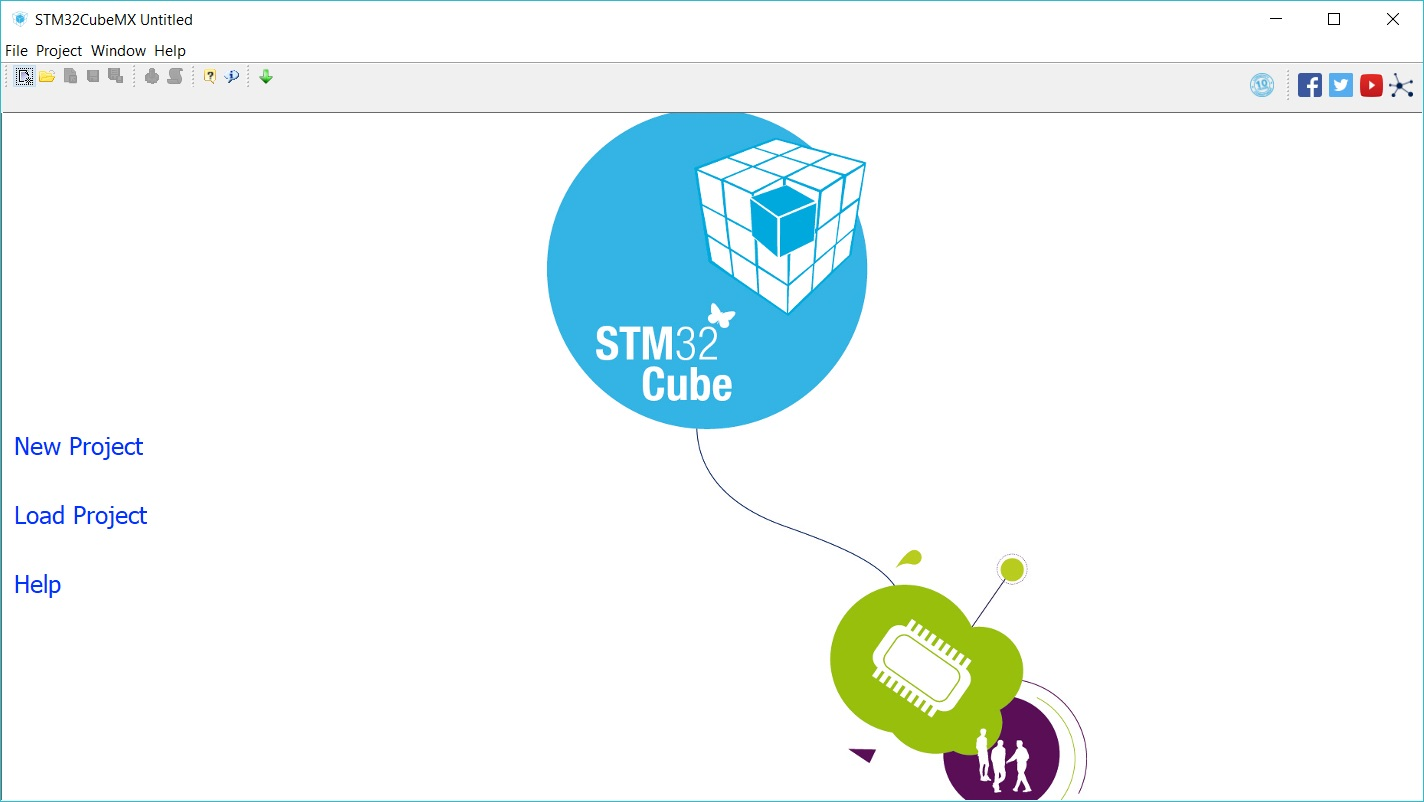
\includegraphics[width=11cm]{STM32CubeMX}
    \caption{Inicializador de proyectos STM32CubeMX}
    \label{fig:STM32CubeMX}
\end{figure}

La herramienta STM32CubeMX incluye una base de datos de todos los microcontroladores disponibles, permitiendo seleccionar el formato, encapsulado e incluso si se va a utilizar en su formato nucleo o en un kit de desarrollo. Incluye también documentación sobre cada microcontrolador y enlaces a distribuidores en caso de que el usuario final quiera comprarlo. 

\subsubsection{Asignación de funciones\label{sec:Configuracion_micro_asignacion}}

Tras seleccionar el microcontrolador, se presenta al usuario una zona de trabajo dividida en cuatro pestañas, cada una destinada a configurar un conjunto de características del microcontrolador: pines y sus funciones, reloj, interfaces de comunicación y consumo de energía.

\begin{figure} [h]
    \centering
    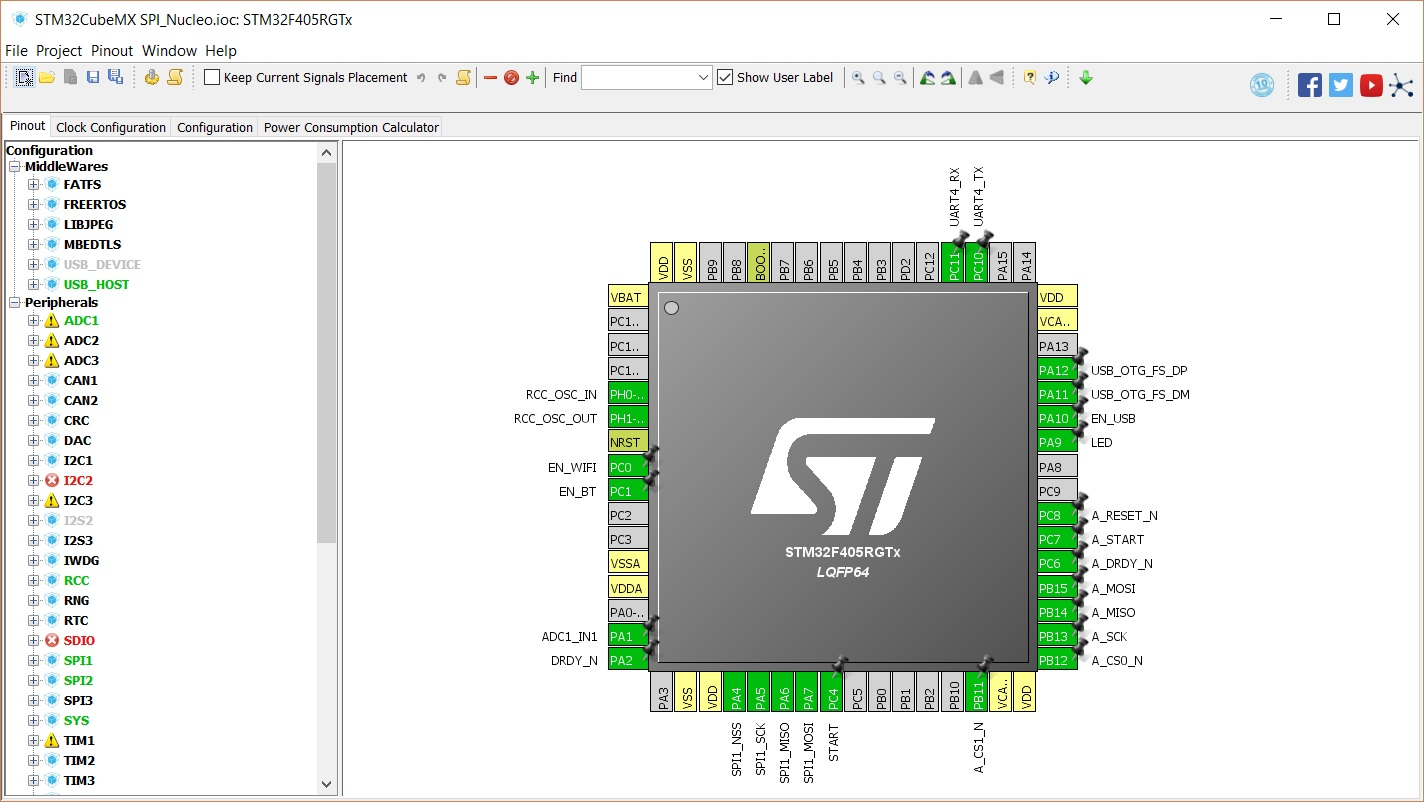
\includegraphics[width=15cm]{STM32CubeMX_pin}
    \caption{Espacio de trabajo del STM32CubeMX}
    \label{fig:STM32CubeMX_pin}
\end{figure}

La configuración de pines permite, no sólo ver de forma visual cada una de las funciones alternativas de cada pin, sino que además indica si alguna no está disponible y las alternativas si se da el caso.

En la figura \ref{fig:STM32CubeMX_pin} aparece la configuración utilizada en este proyecto. En la imagen se puede apreciar que todas las interfaces necesarias para llevar a cabo este proyecto ya han sido asociadas a su pin correspondiente y aún quedan libres casi la mitad de los pines. Esto es un indicador de la versatilidad de este dispositivo.

\subsubsection{Configuración de los relojes\label{sec:Configuracion_micro_reloj}}

Este apartado es el más importante, pues un reloj mal configurado puede provocar errores en la comunicación, una mala gestión del tiempo e incluso que el propio microcontrolador no arranque.

La interfaz desarrollada por STM muestra de forma visual todos los relojes que intervienen en el dispositivo así como las relaciones que hay entre ellos. De esta forma basta con seguir las líneas que conectan los distintos tipos de reloj para saber las dependencias que existen y los resultados que obtendrán en función de los valores escogidos.
\\En caso de que alguna configuración sea incorrecta la propia herramienta está preparada para ofrecer una solución que se acerque lo máximo posible a los resultados deseados.

\begin{figure} [h]
    \centering
    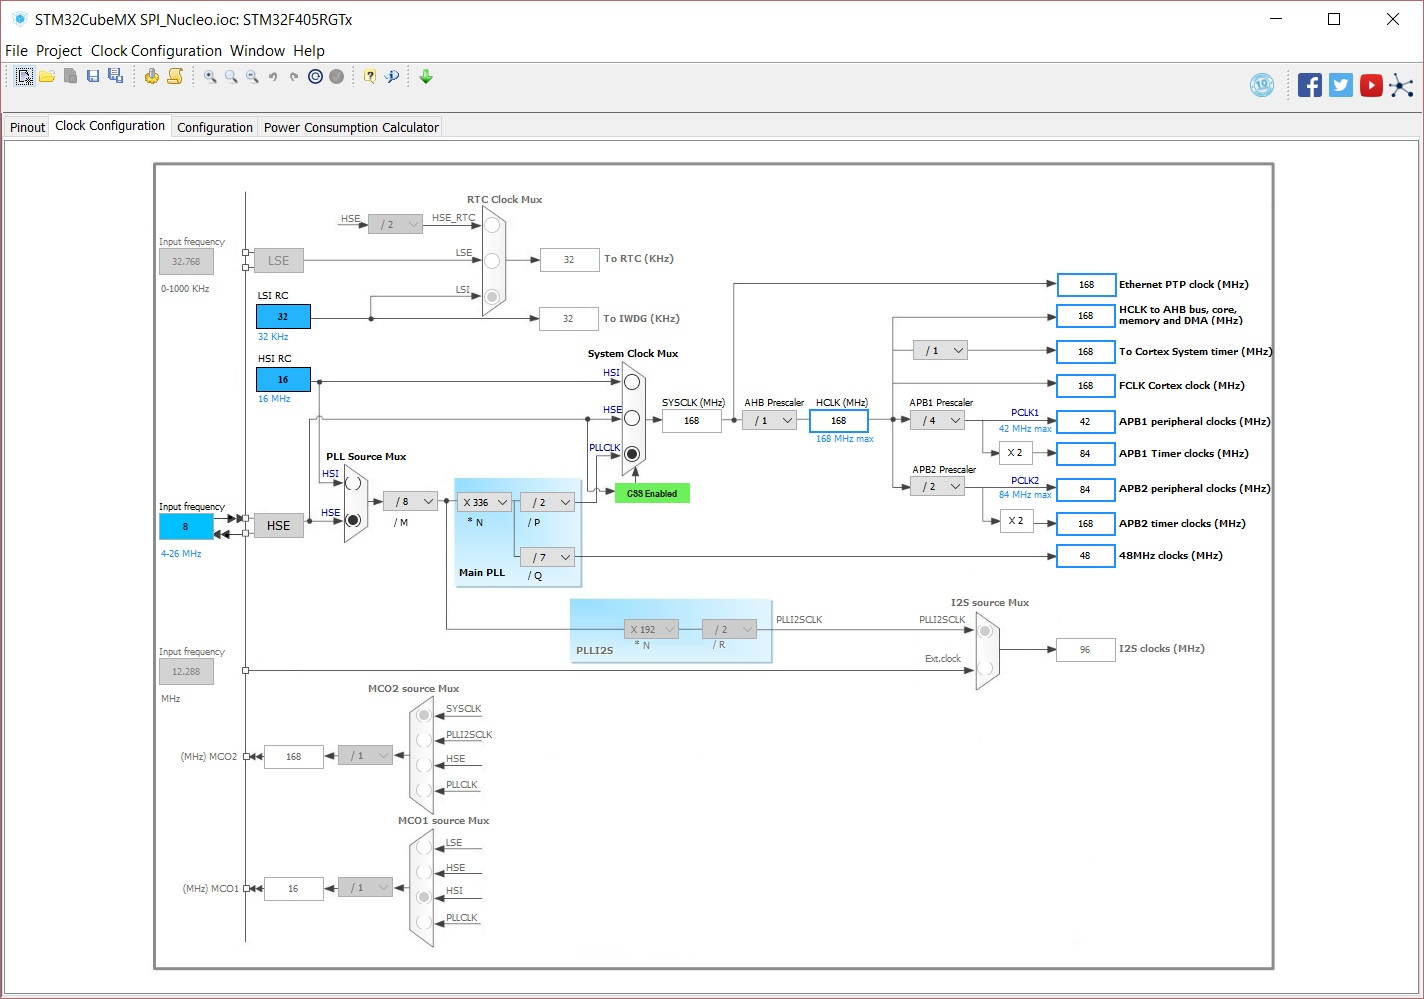
\includegraphics[width=15cm]{STM32CubeMX_clock}
    \caption{Configuración del reloj del microcontrolador}
    \label{fig:STM32CubeMX_clock}
\end{figure}

En la figura \ref{fig:STM32CubeMX_clock} representa la configuración aplicada al microcontrolador durante la realización de este proyecto. A la izquierda se muestran distintas fuentes disponibles mientras que a la derecha se ve la frecuencia final de reloj resultante en cada una de las partes del microcontrolador (periféricos, temporizadores, memoria, etc).

Como se puede ver, aprovecha ambos osciladores, el externo (\acrshort{HSE} = 8MHz) y el interno (\acrshort{LSI} = 16MHz) para, usando \acrshort{PLL}, generar un reloj de una frecuencia mucho más elevada (168 MHz). Dicha frecuencia es, según el fabricante, la máxima frecuencia alcanzable por el dispositivo.

La función \acrshort{CSS} garantiza que, en caso de fallo del reloj del microcontrolador, este generará una alerta y entrará en un modo seguro. Esta función es muy útil cuando se está trabajando con elementos en los que la seguridad de las personas depende directamente del correcto comportamiento microcontrolador.

\clearpage

\subsubsection{Configuración de los periféricos\label{sec:Configuracion_micro_com}}

La tercera pestaña permite configurar los periféricos, esto incluye interfaces de comunicación, puertos GPIO, USB, etc.

\begin{figure} [h]
    \centering
    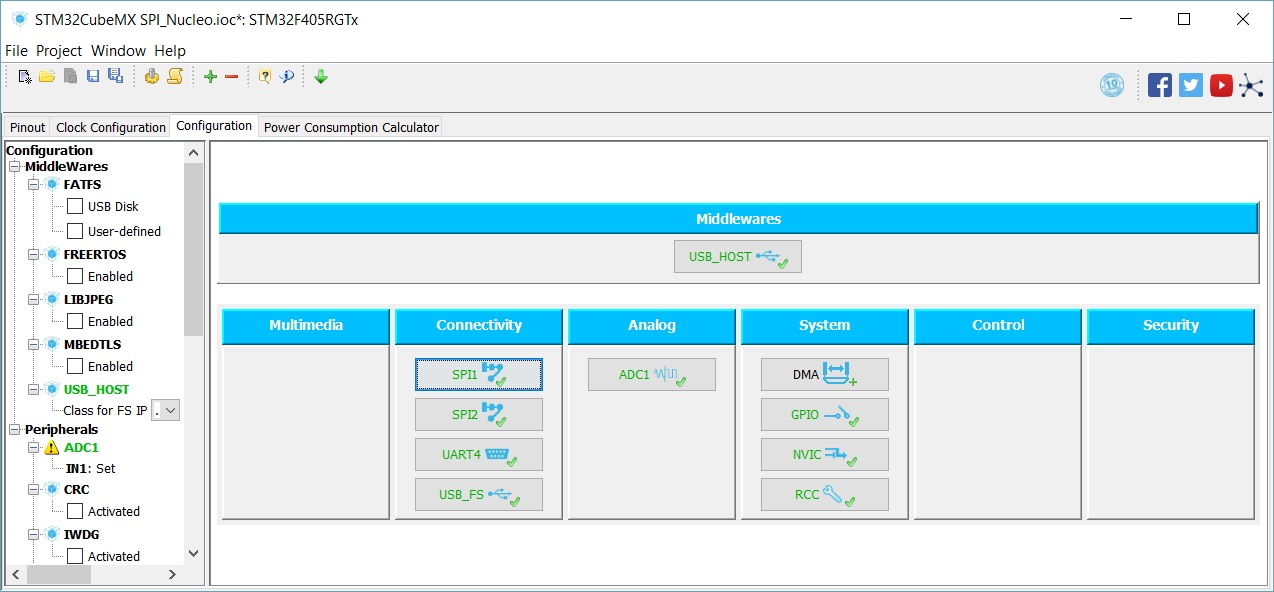
\includegraphics[width=15cm]{STM32CubeMX_conf}
    \caption{Configuración de las interfaces de comunicación}
    \label{fig:STM32CubeMX_conf}
\end{figure}

En función del estado del periférico, este aparecerá marcado con un \textit{tick} verde indicando que todo está correctamente configurado o una cruz roja avisando que alguna característica podría no estar disponible. Además será posible modificar la mayoría de las opciones relacionadas con ese periférico de forma intuitiva. 

\begin{figure} [h]
    \centering
    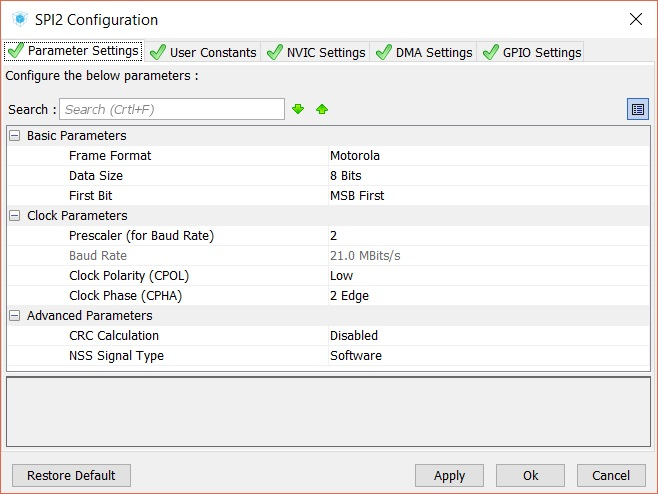
\includegraphics[width=10cm]{STM32CubeMX_conf_2}
    \caption{Detalle de la configuración de las interfaces de comunicación}
    \label{fig:STM32CubeMX_conf_2}
\end{figure}

En la figura \ref{fig:STM32CubeMX_conf_2} se muestran las opciones seleccionadas para el SPI que se comunicará con el los ADS. Se puede cambiar la velocidad, el modo de transmisión e incluso si la gestión del pin ``\textit{Chip-Select}'' se realizará de forma automática o manual.

\subsubsection{Calculo de consumo\label{sec:Configuracion_micro_consumo}}

La última pestaña, ``\textit{Power Consuption Calculator}'', contiene numerosas opciones para el análisis del consumo del microcontrolador. En esta se puede estimar la duración de la batería en función de parámetros como el modo funcionamiento, el tipo de fuente de alimentación e incluso la temperatura.

\begin{figure} [h]
    \centering
    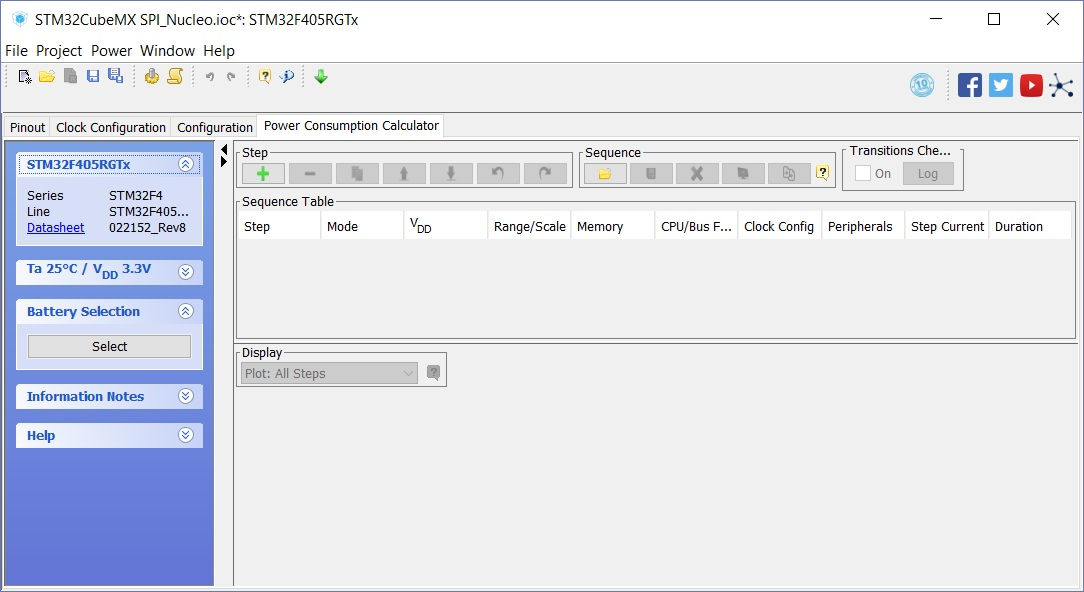
\includegraphics[width=15cm]{STM32CubeMX_otro}
    \caption{Calculadora del consumo del microcontrolador}
    \label{fig:STM32CubeMX_otro}
\end{figure}

\subsubsection{Generar código\label{sec:Configuracion_micro_generador}}

Finalmente es el momento de seleccionar el IDE para el cual el STM32CubeMX debe generar la base de código sobre la que se construirá el proyecto.

Esta herramienta es capaz de crear un código base para casi cualquier \acrshort{IDE} pero tras un par de usos queda claro que, de entre todos los disponibles, es armKeil con el que la integración da mejores resultados. La herramienta crea el código base con la configuración seleccionada desde la interfaz y lo integra dentro de un proyecto ya configurado y listo para trabajar.

Es importante destacar que la utilización de STM32CubeMX no sólo está pensada para facilitar el comienzo del diseño proporcionando una base sobre la que trabajar, también permite una mayor portabilidad del código ya que, si se siguen las reglas de programación sugeridas por la aplicación, esta permite realizar cambios de la configuración de los pines, los periféricos e incluso de familia de microcontrolador, todo ello sin necesidad de reestructurar el código.

\clearpage

El código que se ejecuta en el STM está dividido en dos fases. La primera, denominada comúnmente \textit{setup}, sólo se ejecuta la primera vez que se enciende el microcontrolador.
En esta se suelen declarar todas las variables globales, inicializar los periféricos y, en definitiva, preparar el microcontrolador para funcionar.

La segunda fase, denominada \textit{loop} es, como su nombre indica, un bucle infinito. En esta fase se ejecuta todo el código de forma cíclica. Normalmente en esta fase se incluye el funcionamiento normal del sistema, utilizando condicionales para forzar el comportamiento esperado.

Al generar el proyecto, el STM32CubeMX estructura el código tal como se muestra en el código \ref{algoritmo:Auto_gen}, dejando al usuario ciertas zonas libres para escribir en ellas y restringiendo la escritura en otras.

\begin{lstlisting}[label=algoritmo:Auto_gen,style = STM-code,frame=single,caption=Ejemplo de generación de código automáticamente]
  /* USER CODE BEGIN 1 */
	
  /* USER CODE END 1 */

  /* MCU Configuration----------------------------------------*/

  /* Reset of all peripherals, Initializes the Flash interface and the Systick. */
  HAL_Init();

  /* USER CODE BEGIN Init */

	
  /* USER CODE END Init */
\end{lstlisting}

Respetar dichas restricciones es opcional, pero en caso de no hacerlo no se podrá volver a cambiar la configuración original del micro mediante el STM32CubeMX, pues dicha herramienta las utiliza como referencia y no respetarlas puede ocasionar la pérdida del trabajo.

Por simplicidad, comodidad y compatibilidad, durante la realización de este trabajo se han respetado dichas restricciones construyendo todo el código en las zonas habilitadas para ello.

\clearpage

\subsection{Implementación del firmware \label{sec:Software_micro_HAL}}

A lo largo de las siguientes páginas se presentará una introducción a los elementos software utilizados, haciendo especial hincapié en aquel código cuya función es indispensable para cumplir con las especificaciones fijadas al comienzo del proyecto.

\subsubsection{HAL \label{sec:Software_micro_HAL}}

La programación de microcontroladores basados en Arduino y su \acrshort{IDE} resulta especialmente intuitiva ya que desde sus comienzos ese era uno de los objetivos: acercar el mundo analógico y digital a gente poco iniciada.

Los ARM de STM en cambio, están destinados a personas con cierta experiencia programando controladores. Permiten libertad total, proporcionando acceso a los registros sin restricciones y un control del hardware muy preciso. Si bien esta aproximación aumenta las posibilidades de la plataforma, también limita al número de personas que pueden ponerse a programar en ella así como la portabilidad de código.
\\Cuanto más cercano sea al hardware mayor exclusivo será y, por lo tanto, más cambios serán necesarios para portar dicho código a otra familia si en el futuro las especificaciones varían o se desean mejorar las características del sistema.

Con esta problemática en mente los desarrolladores de STM crearon un conjunto de herramientas y drivers que reciben el nombre de Hardware Abstraction Layer (\acrshort{HAL}).

\begin{figure} [h]
    \centering
    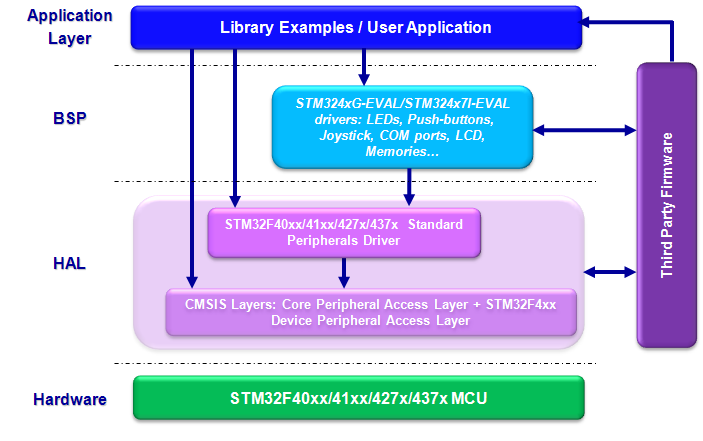
\includegraphics[width=13cm]{HAL-LL}
    \caption{Resumen del funcionamiento y características del HAL \cite{HAL-LL}}
    \label{fig:HAL-LL}
\end{figure}

La utilización de \acrshort{HAL} no sólo permite portar código entre familias de STM sino que simplifica sensiblemente el desarrollo de un proyecto, pues integra un gran número de funciones relacionadas con la gestión de los distintos puertos de comunicaciones y GPIO así como otras encargadas de realizar operaciones matemáticas complejas.

\subsubsection{Estructura del código\label{sec:Software_micro_estados}}

El código está organizado siguiendo el esquema típico de una máquina de estados. Haciendo uso de condicionales de tipo ``switch - case'' se ha construído el programa representado en la figura \ref{fig:Maquina_estados_STM}. 

\begin{figure} [h]
    \centering
    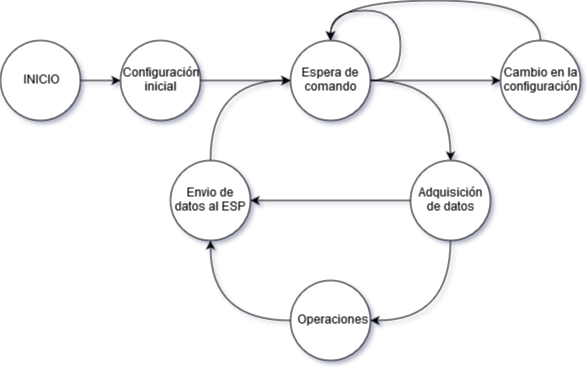
\includegraphics[width=16cm]{Maquina_estados_STM}
    \caption{Estructura del programa}
    \label{fig:Maquina_estados_STM}
\end{figure}

En primer lugar se realiza una inicialización de todas las variables, los periféricos y el resto de dispositivos que se encuentran conectados con el STM.

A continuación, el microcontrolador se queda a la espera de un comando por parte del ESP-12E que le indicará que hacer. Por el momento se han implementado tres alternativas, dos relacionadas con la adquisición de datos y una para cambios de   configuración, pero está preparado para aumentar el número de condiciones con facilidad. De esta forma el software puede aumentar en funcionalidades sin que haya que reestructurar el código.

Si el microcontrolador recibe la orden de adquirir datos, este activa la comunicación SPI y queda a la espera de una confirmación por parte del ADS de que los datos están listos para ser leídos del bus.

Tras leer los datos el microcontrolador convierte la información a formato \textit{float} y calcula la equivalencia en voltaje de la medida. 

Posteriormente, en función de la orden recibida desde el ESP, el STM transmite la información al ESP o bien realiza operaciones matemáticas sobre los datos y finalmente los transmite al ESP. Estas operaciones pueden ser sumas, restas e incluso un filtrado de la señal para eliminar componentes indeseadas.

\subsubsection{Transmisión de datos por SPI \label{sec:Software_micro_SPI}}

Aunque la capa de abstracción del hardware facilita notablemente el trabajo de desarrollo, para poder trabajar con un bus de comunicaciones de forma eficiente y sin errores es necesario saber como funciona a nivel hardware y, desde ahí, realizar una abstracción progresiva. 

En primer lugar será importante definir que elemento hará las funciones de Máster y cual de Esclavo, pues esto limitará las características de la comunicación y forzará la configuración de los \acrshort{GPIO} de una forma u otra.

\begin{figure} [h]
    \centering
    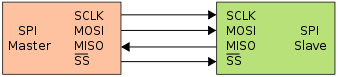
\includegraphics[width=10cm]{SPI_Master_Slave}
    \caption{Esquema de comunicaciones SPI}
    \label{fig:SPI_Master_Slave}
\end{figure}

Para aprovechar la tasa de transferencia del SPI del STM al máximo lo ideal sería que fuese este el Máster en ambas comunicaciones (hacia el ADS y hacia el ESP). Esto es así porque la máxima velocidad de transmisión es definida por el Máster mientras que el Esclavo se adapta a las normas impuestas, siempre dentro de unos rangos establecidos por el fabricante.

Por desgracia, las limitaciones de las librerías disponibles para el ESP-12E fuerzan que este sea obligatoriamente el Máster de esa comunicación limitando la velocidad a la máxima que sea capaz de alcanzar el ESP.

Para la transmisión de datos desde el STM es muy importante tener en cuenta que el microcontrolador trabaja a bajo nivel. Las funciones implementadas en los \textit{drivers} y librerías de abstracción de hardware facilitan el trabajo, pero debe tenerse presente en todo momento que se está transmitiendo información de registros de memoria y, por lo tanto, no se debe perder de vista el tamaño del dato ni el tipo del mismo.

Las funciones encargadas de transmitir información a través del puerto \acrshort{SPI} son:
\begin{itemize}
\item HAL\_StatusTypeDef HAL\_SPI\_Transmit
\item HAL\_StatusTypeDef HAL\_SPI\_Receive
\item HAL\_StatusTypeDef HAL\_SPI\_TransmitReceive
\end{itemize}

Las tres funciones necesitan el puntero al puerto por el que se transmitirá la información, la dirección de memoria de la misma, el tamaño del conjunto de datos y el tiempo de espera por cada transmisión.

El código \ref{algoritmo:STM_Transmision_SPI} muestra la cabecera de la función encargada de transmitir y recibir información de forma simultánea. En el se puede ver con claridad el tipo de datos que necesita para realizar una transmisión de datos de forma satisfactoria.

\begin{lstlisting}[label=algoritmo:STM_Transmision_SPI,style = STM-code,frame=single,caption=Transmisión de datos a través de SPI con el STM]
HAL_StatusTypeDef HAL_SPI_TransmitReceive(
	SPI_HandleTypeDef *hspi,
 	uint8_t *pTxData, 
 	uint8_t *pRxData, 
 	uint16_t Size, 
	uint32_t Timeout)
\end{lstlisting}

Las funciones encargadas de transmitir y recibir información, ya sea a través de SPI o a través de otro periférico, funcionan de forma similar y por lo tanto necesitan las mismas variables. Salta a la vista que, a pesar de que la función simplifica sensiblemente la gestión de memoria y pines, aún es necesario tener en cuenta ciertas limitaciones que marcarán el modo de trabajo:
\begin{itemize}
\item \textbf{Tamaño de transmisión fijo}\\
El tamaño de los datos a transmitir debe ser de 8 bits. En caso de querer transmitir una variable cuyo tamaño en memoria sea superior a este será necesario realizar una transformación.
\item \textbf{Gestión de pines manual o automática}\\
La gestión de pines como ``\textsc{Data-Ready}'' y ``\textsc{Start}'' se debe realizar de forma manual. ``\textsc{Chip-Select}'' en cambio está pensado para gestionarlo de forma manual o automática en función de las circunstancias.
\item \textbf{Gestión de memoria}\\
El STM es capaz de transmitir una gran cantidad de datos por \acrshort{SPI}. Es importante tener claro la cantidad de datos a recibir o transmitir, pues equivocarse puede suponer acceder a una dirección de memoria no permitida, recibir valores incorrectos o incluso corromper el código y forzar el reinicio del microcontrolador.
\end{itemize}

Al ser obligatorio transmitir datos de 8bits se vuelve indispensable crear algún metodo para poder dividir aquellas variables cuyos tamaño sea superior (float, long, etc).
El tipo de dato \textbf{union} definido en \textbf{C} está pensado justo para este cometido. Permite definir varias variables cuyo tamaño total sea equivalente y asignar la misma dirección de memoria a todas ellas. A continuación se muestra un fragmento del código necesario para dividir una variable \textbf{long} (32bits) en un array de 4 posiciones de tipo \textbf{int} (8bits cada una).

\begin{lstlisting}[label=algoritmo:STM_Divisor,style = STM-code,frame=single,caption=División de variables en otras de menor tamaño]
union miDato{
	struct
	{
		uint8_t  b[4];     // Array de bytes de tamaño equivalente
	}split;
		long dato;
} long_data; 
\end{lstlisting}
\clearpage

\subsubsection{Comunicación con el ADS \label{sec:Software_micro_ADS}}

El ADS está preparado para recibir y transmitir información a través del puerto SPI integrado. Aunque puede transmitir información el integrado sólo es capaz de actuar en modo Esclavo y \gls{Full Duplex}. Utilizando el microcontrolador STM como Master es posible comunicar ambos dispositivos a muy altas velocidades.

La memoria del ADS está organizada en distintos registros, cada uno de los cuales con una función definida en la hoja de características del componente. La configuración del dispositivo se realiza de forma casi exclusiva mediante SPI escribiendo directamente sobre el registro deseado.

Al tratarse de registros de memoria, para su modificación resulta indispensable conocer la posición exacta. Aunque para una máquina esto no es un problema, para un ser humano puede resultar complicado recordar e identificar de forma eficiente cada uno de ellos. 
\\Por este motivo se ha creado un archivo ``.h'' con definiciones de todos los registros, asociando cada uno de ellos a un comando. Así por ejemplo la posición de memoria encargada del control de los GPIO en lugar de llamarse escribiendo en el registro 0x14 basta con escribir en el registro \textsc{GPIO}. Con esta transformación se consigue además aumentar la legibilidad del código.

\begin{lstlisting}[label=algoritmo:STM_ADS_def,style = STM-code,frame=single,caption=Ejemplo de definiciones de los registros y funciones del ADS]
//Position in memory of registers: (Pg. 39)

#define ID 						0x00	// (0000 0000)
#define CONFIG1  		 	0x01	// (0000 0001) 
#define CONFIG2  			0x02 	// (0000 0010)
.		.						  .					.
#define CONFIG4   		0x17 	// (0001 0111)
\end{lstlisting}

El manual de funcionamiento del ADS muestra distintas formas de configuración. Es posible leer y/o escribir un registro o varios de forma simultánea con pocos comandos. De acuerdo al manual, para realizar una escritura de un registro es necesario transmitir tres datos al ADS. El primero indicará la dirección de memoria sobre la que se trabajará. El segundo sirve para seleccionar el número de registros a escribir. Por último el tercer dato es el que se almacenará en memoria. La figura \ref{fig:ADS_wreg} muestra una representación de la transmisión de datos llevada a cabo para la escritura de dos registros en el ADS:

\begin{figure} [h]
    \centering
    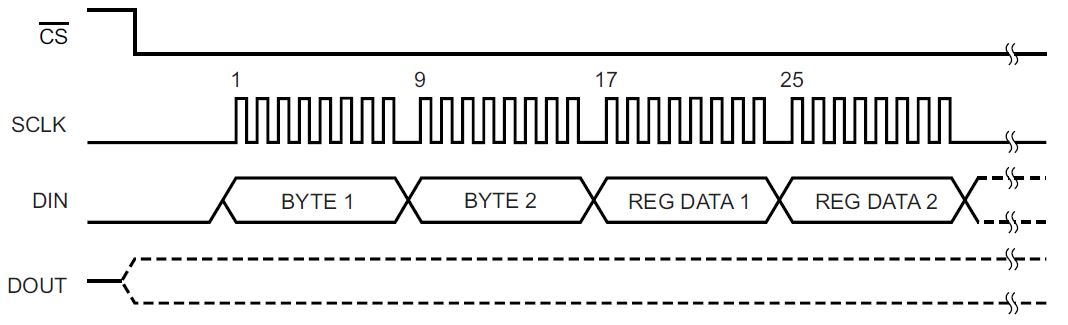
\includegraphics[width=13cm]{ADS_wreg}
    \caption{Escritura de dos registros del ADS \cite{Datasheet_ADS}}
    \label{fig:ADS_wreg}
\end{figure}

El código generado en el STM para realizar esta función es el presentado en \ref{algoritmo:STM_wreg}.

\begin{lstlisting}[label=algoritmo:STM_wreg,style = STM-code,frame=single,caption=Escritura en registros del ADS]
void adc_wreg(uint8_t reg, uint8_t val, SPI_HandleTypeDef *SPI){
	uint8_t zero_t = 0x00;
	uint8_t zero_r = 0x00;
	uint8_t reg_temp = WREG | reg;
	uint8_t val_temp = val;
	
	HAL_GPIO_WritePin(A_CS0_N_GPIO_Port, A_CS0_N_Pin, GPIO_PIN_RESET);
	HAL_SPI_TransmitReceive(SPI, &reg_temp, &zero_r, 1, 100);
	HAL_SPI_TransmitReceive(SPI, &zero_t, &zero_r, 1, 100);	
	HAL_SPI_TransmitReceive(SPI, &val_temp, &zero_r, 1, 100);	

	HAL_Delay(1);
	HAL_GPIO_WritePin(A_CS0_N_GPIO_Port, A_CS0_N_Pin, GPIO_PIN_SET);
}
\end{lstlisting}

La lectura de los registros del ADS se realiza de una forma análoga. En esta ocasión se transmiten los mismos dos datos que para escribir en un registro siendo la única diferencia que el tercer dato (y los siguientes en caso de ser más de un registro) se transmitirán desde el ADS hacia el STM tal y como aparece en la figura \ref{fig:ADS_rreg}.

\begin{figure} [h]
    \centering
    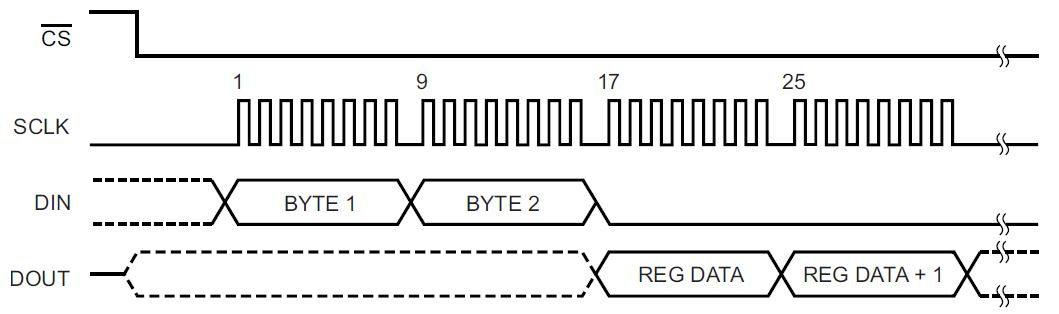
\includegraphics[width=13cm]{ADS_rreg}
    \caption{Lectura de dos registros del ADS \cite{Datasheet_ADS}}
    \label{fig:ADS_rreg}
\end{figure}

\begin{lstlisting}[label=algoritmo:STM_rreg,style = STM-code,frame=single,caption=Lectura de registros del ADS]
uint8_t adc_rreg(uint8_t reg, SPI_HandleTypeDef *SPI){
	uint8_t val = 0x00;
	uint8_t zero_t = 0x00;
	uint8_t zero_r = 0x00;
	uint8_t temp = RREG | reg;
	
	HAL_GPIO_WritePin(A_CS0_N_GPIO_Port, A_CS0_N_Pin, GPIO_PIN_RESET);
	HAL_SPI_TransmitReceive(SPI, &temp, &zero_r, 1, 100);
	HAL_SPI_TransmitReceive(SPI, &zero_t, &zero_r, 1, 100);	
	HAL_SPI_TransmitReceive(SPI, &zero_t, &val, 1, 100);

	HAL_Delay(1);
	HAL_GPIO_WritePin(A_CS0_N_GPIO_Port, A_CS0_N_Pin, GPIO_PIN_SET);

	return val;
}
\end{lstlisting}

Para que la transmisión sea correcta es muy importante que todas las variables definidas sean independientes. Además, el ADS necesita que durante la lectura de datos el pin \textsc{MOSI} se mantenga en un 0 lógico todo el rato.

\subsubsection{Lectura y conversión de datos \label{sec:Software_micro_Datos}}

El ADS está construído utilizando un sistema adquisidor de 8 canales, todos adquiridos de forma simultánea utilizando un sistema $\Delta\Sigma$ de 24 bits y ganancia variable.

Tras adquirir los datos estos son codificados siguiendo el siguiente formato:
\begin{table} [H]
 \centering
 \begin{tabular}{|c|c|}
 \hline 
\textbf{Señal de entrada, V$_{IN}$} &  \multirow{2}{*}{\textbf{Código de salida ideal}}\\ 
 \textbf{(INxP - INxN)} &  \\ 
 \hline 
 +FS & 7FFFFFh\\ 
 \hline 
 +FS$/(2^{23}-1)$ & 000001h \\ 
 \hline 
 0 & 000000h\\ 
 \hline 
 -FS & FFFFFFh\\ 
 \hline 
 +FS$(2^{23}/(2^{23}-1))$ & 800000 \\ 
 \hline 
 \end{tabular} 
 \caption{Equivalencia de voltaje ideal de entrada y código de salida}
 \label{tab:ADS_equivalencia}
\end{table}

La tabla anterior es una modificación de la proporcionada en la hoja de características del ADS corrigiendo algunas pequeñas erratas. La variable ``FS'' corresponde a la escala completa de entrada del ADS. En este caso son 4.5V divididos por la ganancia (G).

Para \textbf{voltajes positivos} la decodificación de estos valores es muy sencilla, pues basta con aplicar una simple \textbf{regla de tres} en la que cada bit es un incremento de $4.5V/(2^{23}*G)$.\\
Para \textbf{voltajes negativos} basta con \textbf{invertir} todos los bits y aplicar la misma regla de tres.\\
El bit más significativo indica si el voltaje final será positivo (0) o negativo (1) y es el que se ha usado como referencia para aplicar la conversión anterior en caso de ser necesaria.

Al trabajar con datos de 24 bits no es posible realizar una inversión directa del valor de la variable o los 8 bits más significativos se verían invertidos también. Por suerte el ADS transmite los datos en paquetes de 8 bits lo cual facilita tratarlos de forma independiente y, tras hacer la transformación a nivel de bit, crear una variable que represente el valor real.

Unir los tres bytes una vez se ha realizado la conversión es posible de múltiples formas. Por motivos de eficiencia y de reutilización del código se ha realizado la misma aproximación ya expuesta previamente haciendo uso de datos de tipo \textbf{union}.

El código \ref{algoritmo:ADS_decodificacion}, incluído en una librería creada para interactuar con el ADS, es el utilizado para este fin.

\clearpage

\begin{lstlisting}[label=algoritmo:ADS_decodificacion,style = STM-code,frame=single,caption=Decodificación de datos binarios a Voltajes]
float32_t byte2float (uint8_t data_23_16, uint8_t data_15_8, uint8_t data_7_0, uint8_t ganancia)
	{
		float32_t value = 0;
		
		union miDato{
		struct
		{
			uint8_t  b[4];     // Array de bytes de tamaño igual al tamaño de la primera variable: int = 2 bytes, float = 4 bytes
		}split;
			long dato;
	 } long_data; 
		
	 long_data.dato = 0;
	 
		if (data_23_16>=0x80) //1000 0000
		{
			long_data.split.b[2] = ~data_23_16;
			long_data.split.b[1] = ~data_15_8;
			long_data.split.b[0] = ~data_7_0;
			value = long_data.dato;
			value = -value;
		}
		else
		{
			long_data.split.b[2] = data_23_16;
			long_data.split.b[1] = data_15_8;
			long_data.split.b[0] = data_7_0;
			value = long_data.dato;
		}
		
		value = value*4.5f/(8388607.0f*ganancia); //4.5/(2^23*G)
		
		return value;
	}
\end{lstlisting}

El código anterior realiza una conversión triple: 4 bytes $\Rightarrow$ long $\Rightarrow$ float, donde el valor final devuelto es el voltaje real medido una vez se ha aplicado el factor de ganancia correspondiente.

El ADS tiene embebido un sistema de control basado en comandos a través de SPI. Estos comandos permiten realizar ciertas operaciones en tiempo real que facilitan el control del integrado y amplian sus características. 

La tabla \ref{tab:ADS_comandos}, sacada de la hoja de características del componente, muestra todos los comandos que el ADS es capaz de reconocer, sus funciones y el conjunto de bytes que representa cada uno. Los últimos dos comandos corresponden a la lectura y escritura en registros y ya han sido explicados previamente.

\begin{table}[H]
    \centering
    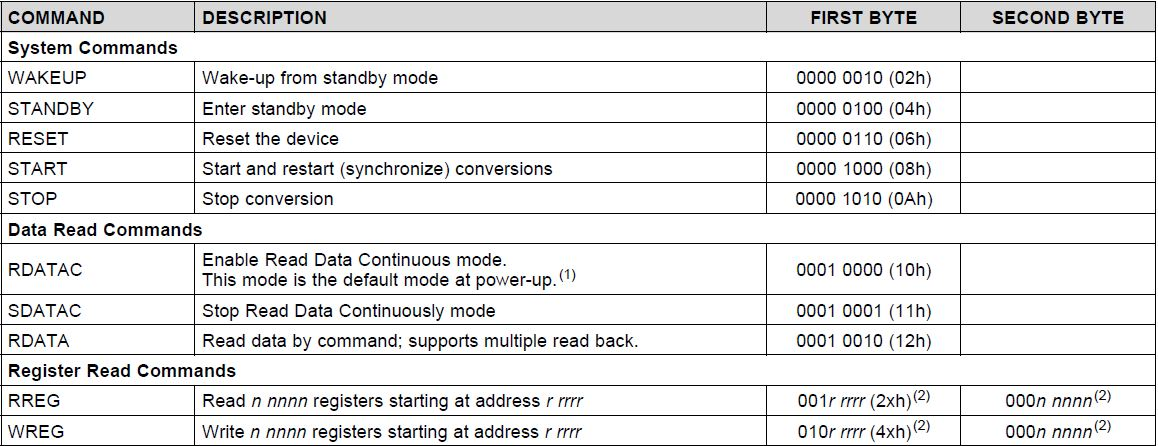
\includegraphics[width=16cm]{ADS_comandos}
    \caption{Comandos del ADS1299}
    \label{tab:ADS_comandos}
\end{table}

Durante la realización de este proyecto ha sido necesario utilizar la mayor parte de los comandos presentados en la tabla anterior. Cabe destacar que aquellos categorizados como ``Comandos del sistema'' han sido necesarios durante la secuencia de inicio del ADS casi en exclusiva, pues no se han implementado funciones de ahorro de energía. Estas se han contemplado como una mejora a llevar a cabo en futuras iteraciones de este proyecto.

El ADS cuenta con dos modos de lectura: continua y bajo demanda. Los comandos categorizados como ``Comandos de lectura'' están relacionados con la gestión de estos dos modos y se dividen a su vez en dos tipos según su función:
\begin{itemize}
\item \textbf{Configuración}\\
\textsc{RDATAC} y \textsc{SDATAC} activan y desactivan el modo de lectura continua respectivamente. El ADS se encuentra por defecto en modo continuo tras completar la secuencia de inicio.
\item \textbf{Lectura}\\
\textsc{RDATA} solicita en el modo de lectura bajo demanda la transmisión de los datos capturados en ese momento.
\end{itemize} 

El modo bajo demanda está pensado para aquellos sistemas en los que es necesario adquirir poca información a lo largo del tiempo. En esta configuración el ADS se mantiene inactivo hasta que recibe el comando de lectura y sólo entonces es cuando la realiza. Este comportamiento favorece la implementación de sistemas de ahorro de energía basados en los comandos \textsc{STANDBY} y \textsc{WAKEUP}. De esta forma es posible aumentar la autonomía del sistema completo considerablemente.

Por desgracia, este modo no es compatible con la transmisión de grandes cantidades de datos o mediciones muy continuas. Por cada medida es necesario utilizar el comando \textsc{RDATA}, afectando directamente al rendimiento y eficiencia en la transmisión.

La figura \ref{fig:ADS_SDATAC} ilustra la transmisión de información usando el modo bajo demanda.

\begin{figure} [H]
    \centering
    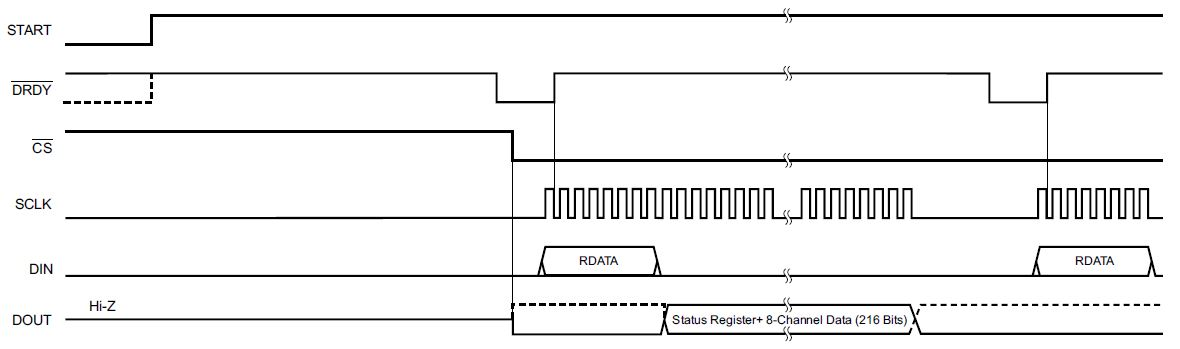
\includegraphics[width=15cm]{ADS_SDATAC}
    \caption{Modo de uso del comando \textsc{RDATA}}
    \label{fig:ADS_SDATAC}
\end{figure}

Por los motivos explicados anteriormente este modo no será utilizado normalmente pero aún así se ha decidido trabajar en su implementación en caso de que fuese necesario en el futuro. El código utilizado para adquirir datos es el siguiente:

\begin{lstlisting}[label=algoritmo:ADS_oneshot,style = STM-code,frame=single,caption=Lectura de datos en modo \textit{one-shot}]
void one_shot (uint8_t data[], SPI_HandleTypeDef *SPI)
{
	uint8_t zero = 0x00;
	uint8_t cmd = RDATA;
			
	while (HAL_GPIO_ReadPin(A_DRDY_N_GPIO_Port, A_DRDY_N_Pin) == GPIO_PIN_SET){}

	HAL_GPIO_WritePin(A_CS0_N_GPIO_Port, A_CS0_N_Pin, GPIO_PIN_RESET);
	
	HAL_SPI_TransmitReceive(SPI, &cmd, &zero,  1, 100);

	read_data_frame(data, SPI);
			
	while (HAL_GPIO_ReadPin(A_DRDY_N_GPIO_Port, A_DRDY_N_Pin) == GPIO_PIN_RESET) {}			
				
	HAL_GPIO_WritePin(A_CS0_N_GPIO_Port, A_CS0_N_Pin, GPIO_PIN_SET);

	update_bias_ref(data, SPI);
}
\end{lstlisting}

Para recibir una gran cantidad de información de forma ininterrumpida el ADS cuenta con el modo continuo. Se transmite el comando \textsc{RDATAC} y desde ese momento el ADS empieza a adquirir información y transmitirla. El pin \textsc{DRDY} es utilizado por el ADS para indicar que la siguiente tanda de datos está disponible para su lectura. 

La figura \ref{fig:ADS_RDATAC} representa la transmisión de información en modo continuo y el código \ref{algoritmo:ADS_continuo} el código equivalente.

\begin{figure} [H]
    \centering
    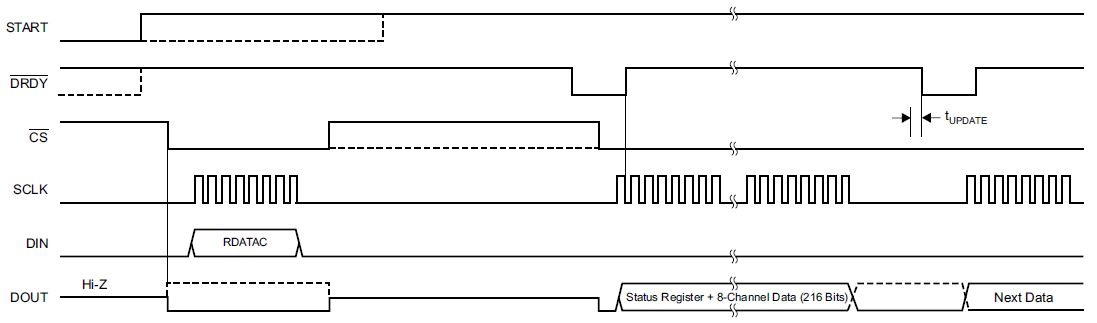
\includegraphics[width=16cm]{ADS_RDATAC}
    \caption{Transmisión de datos en modo continuo}
    \label{fig:ADS_RDATAC}
\end{figure}

\begin{lstlisting}[label=algoritmo:ADS_continuo,style = STM-code,frame=single,caption=Lectura de datos en modo continuo]
void adquire_array_data (uint8_t data[], float32_t channel_1[],float32_t channel_2[],float32_t channel_3[],float32_t channel_4[],float32_t channel_5[],float32_t channel_6[],float32_t channel_7[],float32_t channel_8[], uint8_t gain[], SPI_HandleTypeDef *SPI)
{
	int debug = 255;
	// read LENGTH_SAMPLES samples
		
	adc_send_command(RDATAC, SPI);
		
	while (HAL_GPIO_ReadPin(A_DRDY_N_GPIO_Port, A_DRDY_N_Pin) == GPIO_PIN_SET){}
		
	HAL_GPIO_WritePin(A_CS0_N_GPIO_Port, A_CS0_N_Pin, GPIO_PIN_RESET);
		
	read_data_frame(data, SPI);
			
	channel_1[0]=byte2float(data[1*3], data[1*3+1], data[1*3+2], gain[0]);
	channel_2[0]=byte2float(data[2*3], data[2*3+1], data[2*3+2], gain[1]);
	channel_3[0]=byte2float(data[3*3], data[3*3+1], data[3*3+2], gain[2]);
	channel_4[0]=byte2float(data[4*3], data[4*3+1], data[4*3+2], gain[3]);
	channel_5[0]=byte2float(data[5*3], data[5*3+1], data[5*3+2], gain[4]);
	channel_6[0]=byte2float(data[6*3], data[6*3+1], data[6*3+2], gain[5]);
	channel_7[0]=byte2float(data[7*3], data[7*3+1], data[7*3+2], gain[6]);
	channel_8[0]=byte2float(data[8*3], data[8*3+1], data[8*3+2], gain[7]);
			
	while (HAL_GPIO_ReadPin(A_DRDY_N_GPIO_Port, A_DRDY_N_Pin) == GPIO_PIN_RESET){}
			
	for (int i = 1; i<LENGTH_SAMPLES; i++)
	{
		while (HAL_GPIO_ReadPin(A_DRDY_N_GPIO_Port, A_DRDY_N_Pin) == GPIO_PIN_SET){}
			
		read_data_frame(data, SPI);

		channel_1[i]=byte2float(data[1*3], data[1*3+1], data[1*3+2], gain[0]);
		channel_2[i]=byte2float(data[2*3], data[2*3+1], data[2*3+2], gain[1]);
		channel_3[i]=byte2float(data[3*3], data[3*3+1], data[3*3+2], gain[2]);
		channel_4[i]=byte2float(data[4*3], data[4*3+1], data[4*3+2], gain[3]);
		channel_5[i]=byte2float(data[5*3], data[5*3+1], data[5*3+2], gain[4]);
		channel_6[i]=byte2float(data[6*3], data[6*3+1], data[6*3+2], gain[5]);
		channel_7[i]=byte2float(data[7*3], data[7*3+1], data[7*3+2], gain[6]);
		channel_8[i]=byte2float(data[8*3], data[8*3+1], data[8*3+2], gain[7]);
				
		while (HAL_GPIO_ReadPin(A_DRDY_N_GPIO_Port, A_DRDY_N_Pin) == GPIO_PIN_RESET){}
	}
		
	HAL_GPIO_WritePin(A_CS0_N_GPIO_Port, A_CS0_N_Pin, GPIO_PIN_SET);
}
\end{lstlisting}

El STM no permite trabajar con vectores de varias dimensiones de la misma forma que otros lenguajes de programación, así que para capturar todos los canales ha sido necesario repetir código. A cambio, el escalado del código de un canal a varios se realiza de una forma sencilla e intuitiva. En posteriores revisiones de este proyecto se valorará su sustitución por otro sistema más eficiente.

\subsubsection{DSP - Implementación de filtros \label{sec:Software_micro_DSP}}

Una de las características que diferencian los microcontroladores de esta familia de los de otras es la capacidad de realizar operaciones matemáticas sin que ello repercuta de forma muy significativa en el rendimiento. 

Para facilitar su utilización y unificar a todos los desarrolladores ARM ha creado una librería llamada CMSIS-DSP que engloba todas las funcionalidades de procesado de señal más comunes, optimizando dichos algoritmos para hacerlos lo más eficientes posible.
Esta librería incluye los siguientes tipos de operaciones:

\begin{itemize}
\item Operaciones matemáticas básicas, rápidas y complejas
\item \textbf{Filtrado}
\item Matrices
\item Transformaciones
\item Estadísticas
\item Controladores (PID, senos, etc)
\item Interpolación
\item Apoyo
\end{itemize}

Estas funciones utilizan variables de tipo enteros de 8, 16 y 32 bits y float de 32 bits. En esta ocasión se han utilizado exclusivamente las funciones de filtrado de señal, concretamente aquellas dedicadas a la realización de filtros FIR y su aplicación a señales.

ARM ha puesto a disposición de los consumidores una página web de referencia en la que se puede encontrar una descripción detallada de cada función incluyendo su modo de uso y ejemplos \cite{CMSIS-DSP}.

El filtrado de una señal con un filtro FIR en ARM es un proceso sencillo pero que engloba varias herramientas, pues el diseño del filtro se debe realizar de forma independiente. La función utilizada para este fin es ``arm\_fir\_f32()''. \\
Esta función recibe una señal en formato \textbf{float32\_t} (x[n]), los coeficientes del filtro y la longitud de la ventana y devuelve una señal filtrada (y[n]) con las características deseadas.
\begin{figure} [h]
    \centering
    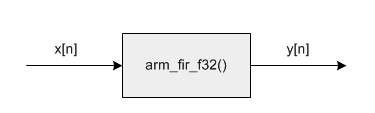
\includegraphics[width=7cm]{arm_fir_f32}
    \caption{Diagrama de bloques del filtrado de una señal x[n]}
    \label{fig:arm_fir_f32}
\end{figure}

El código necesario para aplicar un filtro FIR a una señal es el siguiente:

\begin{lstlisting}[label=algoritmo:STM_filtro,style = STM-code,frame=single,caption=Filtro FIR en STM]
/* ----------------------------------------------------------------------
** Includes necesarios
** ------------------------------------------------------------------- */
#include "arm_math.h"
#include "math_helper.h"
const float32_t firCoeffs32[NUM_TAPS] = {h1, h2, ....,hn}
/* ------------------------------------------------------------------
 * Variables globales para el filtro FIR
 * ------------------------------------------------------------------- */
uint32_t blockSize = BLOCK_SIZE;
uint32_t numBlocks = TEST_LENGTH_SAMPLES/BLOCK_SIZE;
 * ------------------------------------------------------------------- */
arm_fir_instance_f32 S;
arm_status status;
float32_t  *inputF32, *outputF32;
/* Inicialización de buffers de entrada y salida */
inputF32 = &testInput_f32_1kHz_15kHz[0];
outputF32 = &testOutput[0];
/* Inicialización de la estructura de la instancia del filtro FIR. */
arm_fir_init_f32(&S, NUM_TAPS, (float32_t *)&firCoeffs32[0], &firStateF32[0], blockSize);
/* ----------------------------------------------------------------------
** Aplicación del filtro a cada conjunto de blockSize
** ------------------------------------------------------------------- */
for(i=0; i < numBlocks; i++)
{
  arm_fir_f32(&S, inputF32 + (i * blockSize), outputF32 + (i * blockSize), blockSize);
}
\end{lstlisting}

Es una función muy versátil que permite, entre otras cosas, preparar un gran número de filtros y utilizar el más adecuado para cada ocasión sin apenas cambiar el código.

Una de las componentes en frecuencia que más afecta a todas las señales es la de 50 Hz. Para su eliminación se hace uso del equivalente a un filtro \textit{Notch} implementado en un filtro \acrshort{FIR}. Esto se consigue creando un filtro de rechazo de banda lo suficientemente estrecho como para que afecte poco a frecuencias cercanas a la frecuencia a eliminar.

El diseño del filtro se puede hacer con cualquiera de las herramientas disponibles en MatLab. La función ``fir1'' es capaz de definir un filtro con cualquier característica. Tras una primera aproximación con esa función se consiguió un filtro con la respuesta en frecuencia de la figura \ref{fig:FIR_fir1}.
\begin{figure} [H]
    \centering
    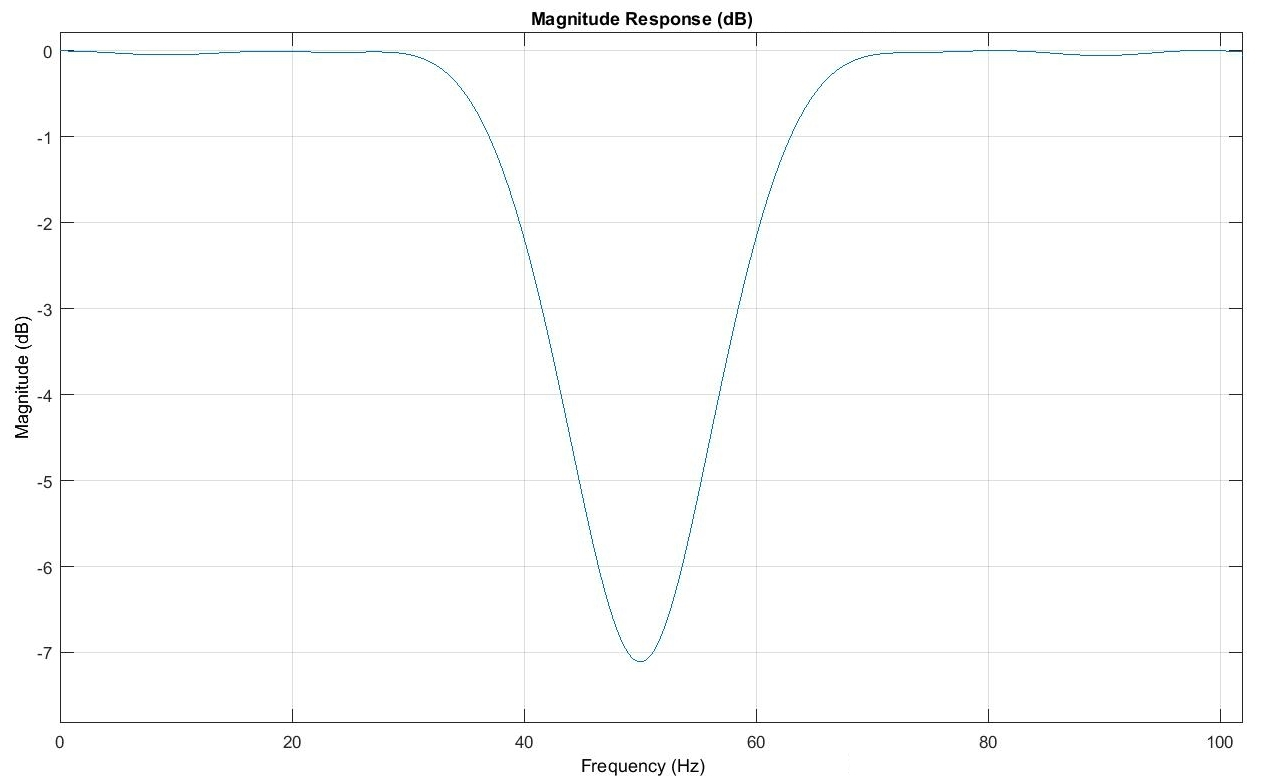
\includegraphics[width=15cm]{FIR_fir1}
    \caption{Respuesta en frecuencia del filtro definido con fir1}
    \label{fig:FIR_fir1}
\end{figure}

Este filtro presenta un comportamiento similar al esperado y un rizado apenas apreciable pero con un factor de rechazo muy bajo. Utilizando otra herramienta diseñada por F.S. Schlindwein disponible en el \textit{workshop} de MatLab es posible ajustar aún más el filtro sin apenas esfuerzo. Tras un par de iteraciones el resultado final fue

\begin{figure} [H]
    \centering
    \includegraphics[width=13cm]{NOTCH_50Hz}
    \caption{CAPTION}
    \label{fig:NOTCH_50Hz}
\end{figure}


Por desgracia la utilización de esta librería provoca que el código supere las limitaciones de la versión gratuita de Keil haciendo necesaria una licencia para poder compilar.

\subsubsection{Comunicación con el ESP \label{sec:Software_micro_ESP}}

El código \ref{algoritmo:STM_Transmision_SPI} es el utilizado para transmitir información al ESP y recibirla.

\begin{lstlisting}[label=algoritmo:STM_Transmision_SPI,style = STM-code,frame=single,caption=Transmisión de datos a través de SPI con el STM]
uint8_t commandFromESP(uint8_t command, SPI_HandleTypeDef *hspi1)
{
	uint8_t response = 0x00;	

		HAL_GPIO_WritePin(DRDY_N_GPIO_Port,DRDY_N_Pin, GPIO_PIN_RESET);
		HAL_SPI_TransmitReceive(hspi1, &command, &response, 1, 100);
		HAL_GPIO_WritePin(DRDY_N_GPIO_Port,DRDY_N_Pin, GPIO_PIN_SET);
		HAL_GPIO_TogglePin(LED_GPIO_Port,LED_Pin); 	//LED OFF
		HAL_Delay(50);
	
	return response;
}
\end{lstlisting}

\subsubsection{Programación del microcontrolador\label{sec:Software_micro_ESP}}

%Software
%Microcontrolador STM
%	CubeMX
%	HAL
%	Implementación del Firmware
%		Maquina de estados
%		Transmisión de datos por SPI
%		Comunicación con ADS
%		Lectura y conversión de datos
%		DSP - Implementación de filtros
%		Comunicación con el ESP
%		
%Microcontrolador ESP
%	Arduino
%	Configuración 
%	Firmware
%		Maquina de estados
%		Transmisión de datos por SPI
%		Comunicación con el STM
%
%LabView


%
% Resultados
%
\chapter{Resultados\label{sec:Resultados}}

En el presente capítulo se han recopilado los resultados obtenidos tras cada una de las fases del proyecto. Por motivos de comprensión y presentación, aquellos resultados asociados al desarrollo de la \acrshort{PCB} han sido presentados en el capítulo \ref{sec:Implementacion_PCB} de modo que no se volverán a repetir en este. En caso de que se deseen revisar de nuevo se crea un enlace a continuación al apartado \ref{sec:PCB_Resultados}.

Los siguientes apartados contienen aquellos resultados asociados al desarrollo del software tanto del microcontrolador STM32F4 como del ESP y su comunicación con LabView.

\section{Funcionamiento del ADS\label{Resultados_ADS}}

Para comprobar que el ADS está midiendo correctamente este incluye una señal de \textit{test} conocida cuyas características se encuentran perfectamente definidas en la hoja de características del componente.

Las características de la señal \textit{test} dependen de los bits almacenados en el registro \textbf{Config 2}. Durante la realización de este proyecto se le ha asignado a Config 2 el valor 0xD1 (11010001) para que la señal de \textit{test} se genere de forma interna, con un voltaje que oscila entre $\pm4.5/2400V$ ($\pm1.875mV$) y frecuencia de f$_\text{CLK}$\/$2^{20}$.

La siguiente figura muestra una representación del voltaje real de la señal test comparándolo con la amplitud teórica calculada según la fórmula proporcionada por la hoja de características:

\begin{figure} [H]
    \centering
    \includegraphics[width=16cm]{Test_teorica}
    \caption{Comparativa entre la señal test y su amplitud teórica}
    \label{fig:tes_teorica}
\end{figure}

Finalmente, tras realizar una medida desde Labview el resultado es el siguiente:

\begin{figure} [H]
    \centering
    \includegraphics[width=15cm]{Test_limpia}
    \caption{Señal de test medida usando LabView}
    \label{fig:Test_limpia}
\end{figure}

Tras comprobar que se recibe una señal con las características esperadas se puede concluir que el ADS se encuentra correctamente configurado y listo para realizar medidas sobre voltajes reales.

\section{Medidas sobre señales reales\label{Resultados_Medida_Real}}

Las primeras señales reales a medir han sido señales con características conocidas. De esta forma resulta muy sencillo identificar si algún elemento no está funcionando correctamente. Para una prueba inicial se preparó un generador de señales haciendo uso de un Arduino UNO. Esta señal presenta una amplitud que va entre 0V y 5V y una frecuencia de 2Hz. El resultado tras medir esta señal se encuentra representado en la figura \ref{fig:Senal_triangular_saturada}.

\begin{figure} [H]
    \centering
    \includegraphics[width=11cm]{Senal_triangular_saturada}
    \caption{Señal real triangular generada con Arduino}
    \label{fig:Senal_triangular_saturada}
\end{figure}

Todos los parámetros se encuentran dentro de los rangos esperados, pero se aprecia una deformación en la señal en los picos superiores del triángulo. Este efecto es debido a la saturación del sistema, pues la amplitud máxima que es capaz de adquirir tanto en positivo como en negativo depende directamente de V$_{\text{REF}}$ (4.5V).

\clearpage

\section{Filtrado de la señal\label{Resultados_filtrado}}

El siguiente paso es aplicar a esas señales reales un filtrado para comprobar que los filtros implementados cumplen con su función.

Siguiendo el ejemplo sugerido por la referencia de CMSIS-DSP se implementó un filtrado de rechazo de banda con el que eliminar las componentes en frecuencia no deseadas de una señal. La señal original es una señal artificial formada por dos senos de distintas frecuencias (10Hz y 50Hz) y el objetivo es eliminar la componente de 50Hz o minimizar su impacto. 

En primer lugar se realizó una estimación del efecto que tendría aplicar un filtro sobre una señal de esas características. El resultadode la simulación realizada en MatLab es el mostrado en la figura \ref{fig:Notch_Matlab}

\begin{figure} [h]
    \centering
    \includegraphics[width=16cm]{Notch_Matlab}
    \caption{Simulación del efecto del filtro Notch a 50Hz}
    \label{fig:Notch_Matlab}
\end{figure}

Como se puede observar, la componente de 50Hz ha sido eliminada casi por completo a costa de afectar ligeramente a la amplitud de la señal original. Tras comprobar que el resultado es satisfactorio se procedió a realizar una implementación del mismo filtro haciendo uso de CMSIS-DSP y el microcontrolador STM32F4.

Al no contarse con generadores de señales capaces de producir una señal de estas características se optó por generar una señal artificial con MatLab y almacenarla en la memoria del STM en la fase de programación. La figura \ref{fig:Filtro_en_STM} muestra la señal original (a) y la señal tras aplicarle el filtro (b).

\begin{figure}[H]
  \begin{subfigure}[b]{8cm}
   	\centering
    \includegraphics[width=8cm]{senal_original}
    \caption{Señal original con ruido de 50Hz}
    \label{fig:senal_original}
  \end{subfigure}
  \hfill
  \begin{subfigure}[b]{8cm}
  	\centering
    \includegraphics[width=8cm]{senal_filtrada}
    \caption{Señal filtrada}
    \label{fig:senal_original}
  \end{subfigure}
  \caption{Implementación real del efecto del filtro Notch a 50Hz}
  \label{fig:Filtro_en_STM}
\end{figure}

Tal y como se esperaba, la señal de 50Hz ha sido eliminada completamente, siendo los resultados obtenidos prácticamente idénticos a los simulados.

El diseño del filtro fuerza a que las componentes en frecuencia cercanas a 50Hz se vean más atenuadas que aquellas más alejadas. Las siguientes figuras muestran señales de 5Hz, 10Hz, 50Hz y 65Hz y como el cambio de frecuencia afecta a la amplitud de la señal.

\begin{figure} [H]
    \centering
    \includegraphics[width=15cm]{seno_5Hz}
    \caption{Señal de 5Hz filtrada}
    \label{fig:seno_5Hz}
\end{figure}

\begin{figure} [H]
    \centering
    \includegraphics[width=15cm]{seno_10Hz}
    \caption{Señal de 10Hz filtrada}
    \label{fig:seno_10Hz}
\end{figure}

\begin{figure} [H]
    \centering
    \includegraphics[width=15cm]{seno_50Hz}
    \caption{Señal de 50Hz filtrada}
    \label{fig:seno_50Hz}
\end{figure}

\begin{figure} [H]
    \centering
    \includegraphics[width=15cm]{seno_65Hz}
    \caption{Señal de 65Hz filtrada}
    \label{fig:seno_65Hz}
\end{figure}

El sistema está cumpliendo su función, pues ha atenuando claramente la señal de 50Hz mientras que las demás se mantienen con una amplitud similar a la original.

\clearpage

\section{Medida de un EEG real\label{Resultados_EEG}}

Las siguientes figuras representan un EEG medido usando la placa de adquisición tras el filtrado de la componente de 50Hz.

\begin{figure} [H]
    \centering
    \includegraphics[width=15cm]{Medida_real_1}
    \caption{EEG abriendo los ojos}
    \label{fig:Medida_real_1}
\end{figure}

\begin{figure} [H]
    \centering
    \includegraphics[width=15cm]{Medida_real_2}
    \caption{EEG con los ojos cerrados}
    \label{fig:Medida_real_2}
\end{figure}

A pesar del filtrado que se ha implementado aún se sigue observando una fuerte componente en frecuencias cercanas a los 50Hz. Esto se debe en gran parte a los sistemas de medida utilizados, ya que la presencia de cables tan largos, finos y con tan poco blindado los convierte en antenas perfectas para captar ruido de esa frecuencia. 

La figura \ref{fig:Sistema_medida} muestra el sistema de medida utilizado para adquirir estas señales.

\begin{figure} [h]
    \centering
    \includegraphics[width=10cm]{usuario_con_diadema}
    \caption{Sistema de medida utilizado para la adquisición del EEG}
    \label{fig:Sistema_medida}
\end{figure}

\section{Transmisión de datos por WiFi\label{Resultados_UDP}}

Por último se incluirán los resultados obtenidos mediante la transmisión de información por TCP y UDP a través de WiFi.

La librería WiFi del ESP contienen un gran número de funciones relacionadas con la transmisión de información tanto por UDP como por TCP.
Con el objetivo de transmitir los datos de la forma más fiable posible se optó por transmitirlos a través de TCP, pues este protocolo tiene sistemas que aseguran que el paquete llegará al destino.

Sin embargo utilizar este protocolo se tradujo en un tiempo de transmisión por cada 250 muestras superior a los 2 minutos haciendo inviable su uso.

En vista de la eficiencia de transmisión conseguida con TCP se utilizó UDP para la transmisión de la información al ordenador. Haciendo uso de este sistema la transmisión se completaba en apenas 1 segundo pero no todos los paquetes llegaban. Tras un poco de investigación se observó que cuanto mayor fuese el retardo introducido entre paquetes menos paquetes se perdían así que se afinó la transmisión hasta conseguir una tasa de transferencia lo suficientemente rápida con una pérdida de paquetes mínima.

\clearpage

En las siguientes imágenes se muestran tres casos en los que se transmitieron 100 paquetes que contenían variables de tipo float, el retardo utilizado entre paquetes y el porcentaje de paquetes perdidos.

\begin{figure}[h]
\centering
  \begin{subfigure}[b]{7cm}
   	\centering
    \includegraphics[width=7cm]{UDP_FAST_LOST}
    \caption{Sin retardo, 92\%}
    \label{fig:UDP_FAST_LOST}
  \end{subfigure}
  \begin{subfigure}[b]{7cm}
  	\centering
    \includegraphics[width=7cm]{UDP_MEDIUM_MEDIUM}
    \caption{Retardo de 1ms, 10\%}
    \label{fig:UDP_MEDIUM_MEDIUM}
  \end{subfigure}
    \begin{subfigure}[b]{7cm}
  	\centering
    \includegraphics[width=7cm]{UDP_SLOW_LOW}
    \caption{Retardo de 5ms, sin pérdidas}
    \label{fig:UDP_SLOW_LOW}
  \end{subfigure}
  \caption{Comparativa entre los distintos retardos y el porcentaje de paquetes perdidos}
  \label{fig:LABEL}
\end{figure}

Con esta información se deduce que para que se reciban todas las muestras que se adquieren por segundo el tiempo de transmisión asciende a 1.25s (250 muestras * 0.005 segundos/muestra).

Este sistema sería ideal si entre transmisiones el sistema de adquisición capturase la siguiente muestra, pues permitiría montar un sistema de adquisición contínuo. Por desgracia esto no es compatible con el filtrado de la señal, al menos no directamente. Además la posibilidad de perder muestras es una característica no deseable.

Finalmente se realizó una segunda iteración sobre TCP, revisando en profundidad las librerías se detectó un error que provocaba un aumento en el tiempo de transmisión muy elevado (es importante recordar que dichas librerías no son oficiales y están en constante desarrollo por lo que la presencia de errores menores es algo habitual). Tras solventar dicho error el tiempo de transmisión de 250 muestras bajó a 1.28 segundos.

El resultado final es muy cercano al conseguido con UDP sin la posibilidad de perder muestras como ocurría con ese protocolo.

%
% Conclusiones
%
\chapter{Conclusiones\label{sec:conclusiones}}

Para la realización de este proyecto ha sido necesario aplicar conocimientos relacionados con casi todas las ramas de las telecomunicaciones.

La rama electrónica es claramente la dominante durante la realización del proyecto, pues el diseño del esquemático, la \acrshort{PCB}, y el montaje de todo el sistema sería imposible sin los conocimientos adquiridos durante mi estancia en la Universidad. Aun así es posible apreciar ciertos matices relacionados con el resto de las ramas, gestión de redes, protocolos de comunicación y el filtrado de las señales han sido utilizados para conseguir los resultados ya mostrados.

El diseño de la \acrshort{PCB} fue muy interesante ya que hasta este momento todos los diseños realizados habían sido orientados al análisis teórico y simulaciones, dejando de lado la implementación final de un sistema de esas características.

Una de las partes del proyecto que más trabajo ha supuesto y que menos se ve reflejado en esta memoria o en el resultado final es el desarrollo del firmware del microcontrolador STM32F4. Este microcontrolador tiene una gran comunidad que lo respalda y un buen número de referencias, pero carece de un sistema de aprendizaje autónomo o guías de iniciación. Esto provoca que el comienzo del desarrollo resulte especialmente complicado.

El sistema ha cumplido ampliamente con las características esperadas. Por supuesto todo es mejorable, no se debe olvidar que este sistema es un prototipo inicial y que no se había trabajado antes con ciertos elementos que juegan un papel principal.

\clearpage

\section{Futuras mejoras}

En futuras iteraciones sobre este proyecto sería deseable ampliar las características ya presentes dotando al sistema de ciertas funciones que no se han implementado por falta de tiempo, y recursos.\\
Algunas de estas características son la adquisición en tiempo real, la parametrización del número de muestras y los tipos de filtros, la inclusión en el software de un sistema de almacenamiento integrado (ya contemplado en el hardware). Igualmente, añadir el sistema de debug por \textsc{\acrshort{jtag}} facilitaría el desarrollo del firmware del microcontrolador.

La mejora más importante podría ser el desarrollo de una \acrshort{PCB} en la que se encuentren todos los elementos integrados, aumentando la comodidad al trabajar con el sistema y su portabilidad.


 

%
% Glosario
%
\printglossary[title=Glosario,toctitle=Glosario]
\printglossary[title=Acrónimos,toctitle=Acrónimos,type=\acronymtype]
%
% Página en blanco
%
\cleardoublepage

%
% Bibliografía
%
%\include{src/Bibliografia}
\nocite{*}
\printbibliography[heading=bibintoc]

% No expandir elementos para llenar toda la página
\raggedbottom

%
% Apéndices
%
\appendix
\cleardoublepage
\addappheadtotoc
\appendixpage

%
% TODO: Apéndices del TFM
%
\chapter{Ejemplos de bloques y comandos útiles en LaTeX\label{sec:ejemplos}}
\section{Ejemplo de sección}

%
% Breve guía de comandos útiles para la memoria
%

% Citar una referencia
%La DARPA creó el protocolo de Internet \cite{ipv4sta}.

% Citar un elemento del glosario
Citamos el acrónimo \gls{PCB}.

% Citar un elemento del glosario (primera letra en may´usculas)
\Gls{bitstream} es una secuencia de bits.

% Insertar una imagen con pie de página
\begin{figure}[htp!]
  \centering
  \includegraphics[width=0.75\textwidth,clip=true]{logo_politecnica}
  \caption{Logo de la Universidad Politécnica de madrid.}
  \label{fig:logo_uam}
\end{figure} 

% Referenciar una etiqueta (label)
La figura~\ref{fig:logo_uam} se utiliza en la portada.

% Nueva página
\clearpage

% Añadir código fuente sin líneas
\begin{lstlisting}[label=algoritmo:quicksort,language=C,frame=single,caption=Algoritmo de ordenación Quicksort]
#include <stdio.h>
 
void quick_sort (int *a, int n) {
    int i, j, p, t;
    if (n < 2)
        return;
    p = a[n / 2];
    for (i = 0, j = n - 1;; i++, j--) {
        while (a[i] < p)
            i++;
        while (p < a[j])
            j--;
        if (i >= j)
            break;
        t = a[i];
        a[i] = a[j];
        a[j] = t;
    }
    quick_sort(a, i);
    quick_sort(a + i, n - i);
}
\end{lstlisting}

% Bloque de código inseparable
\begin{code}
#include <stdio.h>
 
void quick_sort (int *a, int n) {
    int i, j, p, t;
    if (n < 2)
        return;
    p = a[n / 2];
    for (i = 0, j = n - 1;; i++, j--) {
        while (a[i] < p)
            i++;
        while (p < a[j])
            j--;
        if (i >= j)
            break;
        t = a[i];
        a[i] = a[j];
        a[j] = t;
    }
    quick_sort(a, i);
    quick_sort(a + i, n - i);
}
\end{code}

% Fórmula dentro de una línea de texto
La ecuación de Euler ($e^{ \pm i\theta } = \cos \theta \pm i\sin \theta$) es citada frecuentemente como un ejemplo de belleza matemática.

% Fórmula independiente
\begin{equation}\label{eq:pythagoras}
a^2 + b^2 = c^2
\end{equation}


\begin{lstlisting}[language=Python, caption=Python example]
import numpy as np
    
def incmatrix(genl1,genl2):
    m = len(genl1)
    n = len(genl2)
    M = None #to become the incidence matrix
    VT = np.zeros((n*m,1), int)  #dummy variable
    
    #compute the bitwise xor matrix
    M1 = bitxormatrix(genl1)
    M2 = np.triu(bitxormatrix(genl2),1) 

    for i in range(m-1):
        for j in range(i+1, m):
            [r,c] = np.where(M2 == M1[i,j])
            for k in range(len(r)):
                VT[(i)*n + r[k]] = 1;
                VT[(i)*n + c[k]] = 1;
                VT[(j)*n + r[k]] = 1;
                VT[(j)*n + c[k]] = 1;
                
                if M is None:
                    M = np.copy(VT)
                else:
                    M = np.concatenate((M, VT), 1)
                
                VT = np.zeros((n*m,1), int)
\end{lstlisting}

\lstlistoflistings


%AÑADIR DE ANEXO EL BOM

% Fin del documento
\end{document}
